\documentclass[12pt]{report}

% General includes
\usepackage{amsfonts, amssymb, amsmath}
\usepackage{graphicx}
\usepackage{float}
\usepackage{color, soul}
\usepackage{hyperref}

% Font settings
%\renewcommand\familydefault{\sfdefault}
\usepackage{palatino}  % serif
\usepackage{helvet}    % sans-serif
\usepackage{courier}   % typewriter
\usepackage{euler}     % math mode

% Margin and paragraph indent
\usepackage[margin=1.0in]{geometry}
\usepackage{parskip}
\usepackage{tabto}

%\geometry{paperwidth=30cm}
%\geometry{paperheight=40cm}


\begin{document}
\begin{titlepage}
	\centering
	\vspace{1cm}
	{\scshape\Large ESE 370: Circuit-Level Optimization for Digital Systems\par}
	\vspace{1.5cm}
	{\huge\bfseries Project 2 Milestone: FIFO Queue\par}
	\vspace{2cm}
	{\Large\itshape Mauricio Mutai, Jack Harkins\par}
	\vfill
	Instructor: Dr. Tania Khanna\par
	TA: Martin Deng\par
	Date: 11/26/16

	\vfill

% Bottom of the page
	{\large \today\par}
\end{titlepage}

\section*{Design Schematics}
\subsection*{Top-Level Design}
\begin{figure}[H]
  \centering
    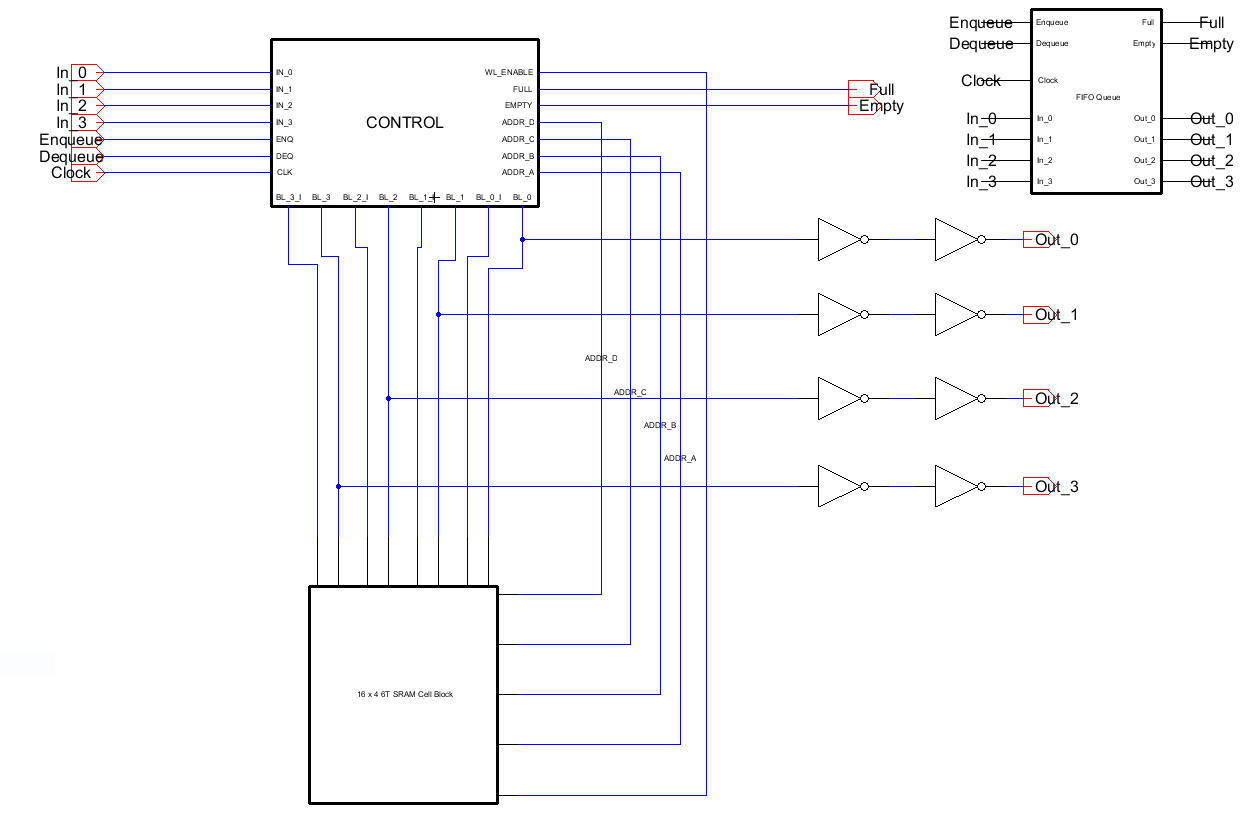
\includegraphics[width=1.0\textwidth]{Schematics/queue_toplevel_schematic.PNG}
  \caption{Queue top-level schematic}
  \label{fig:queue_toplevel_schematic}
\end{figure}

\subsection*{Memory Cell Block}
\begin{figure}[H]
  \centering
    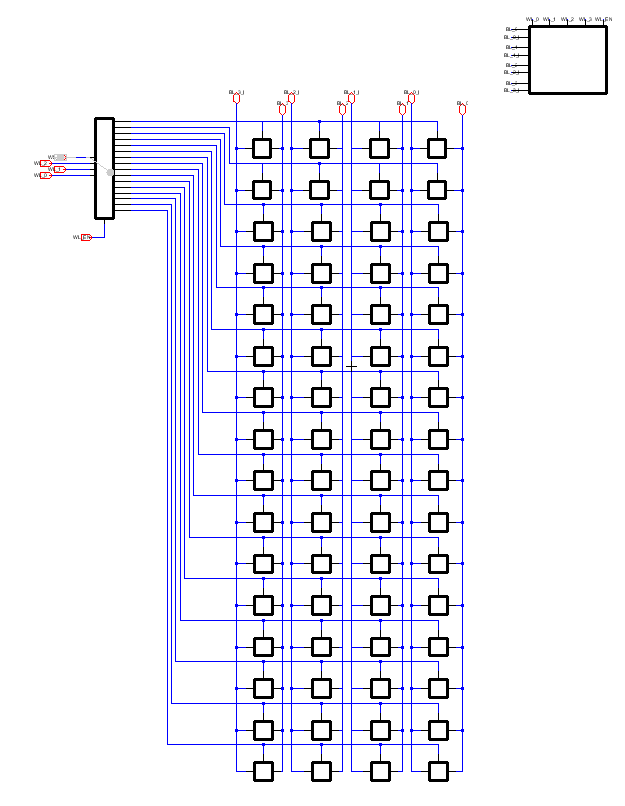
\includegraphics[width=1.0\textwidth]{Schematics/memory_block_allcomponents_schematic.PNG}
  \caption{Memory block toplevel schematic}
  \label{fig:memory_block_allcomponents_schematic}
\end{figure}
\begin{figure}[H]
  \centering
    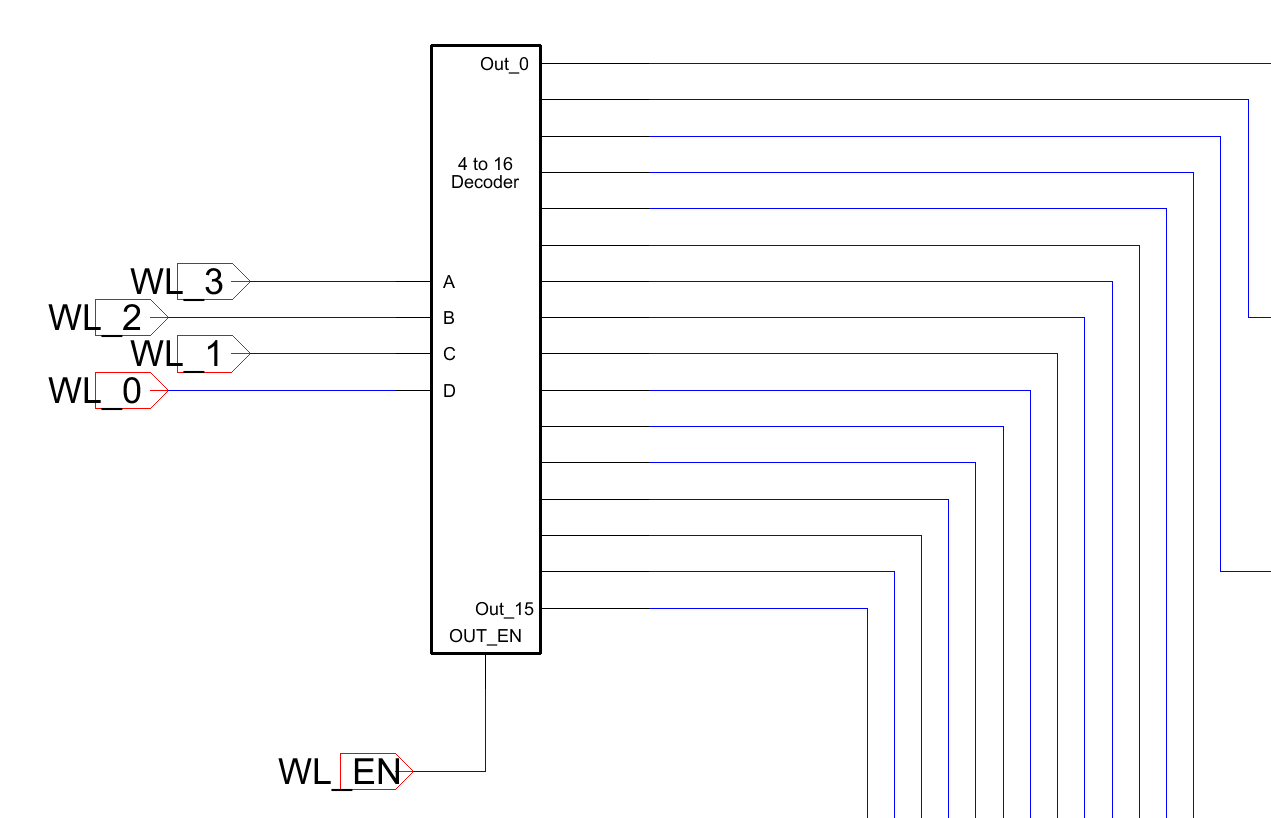
\includegraphics[width=1.0\textwidth]{Schematics/memory_block_decoder_schematic.PNG}
  \caption{Memory block schematic in detail, decoder}
  \label{fig:memory_block_decoder_schematic}
\end{figure}
\begin{figure}[H]
  \centering
    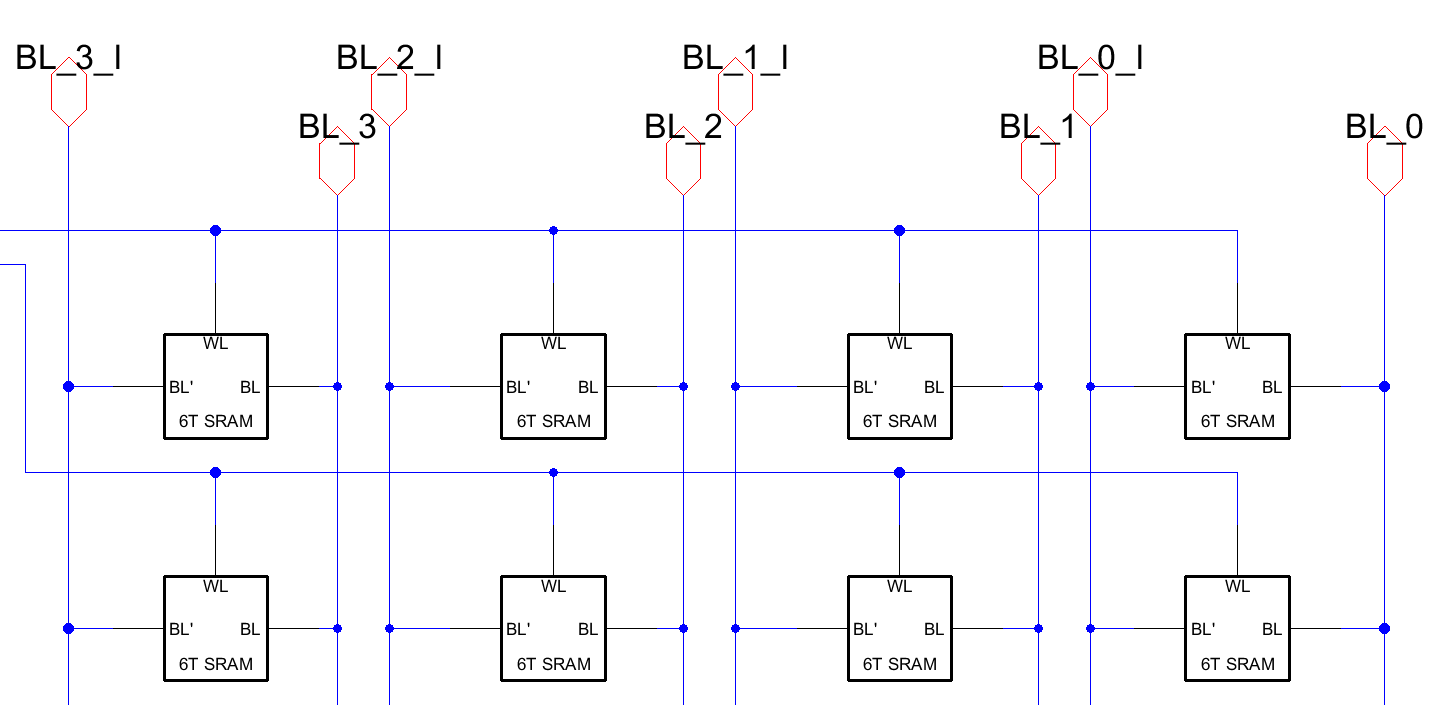
\includegraphics[width=1.0\textwidth]{Schematics/memory_block_word_schematic.PNG}
  \caption{Memory block schematic in detail, word slice}
  \label{fig:memory_block_word_schematic}
\end{figure}

\subsection*{6T SRAM Cell}
\begin{figure}[H]
  \centering
    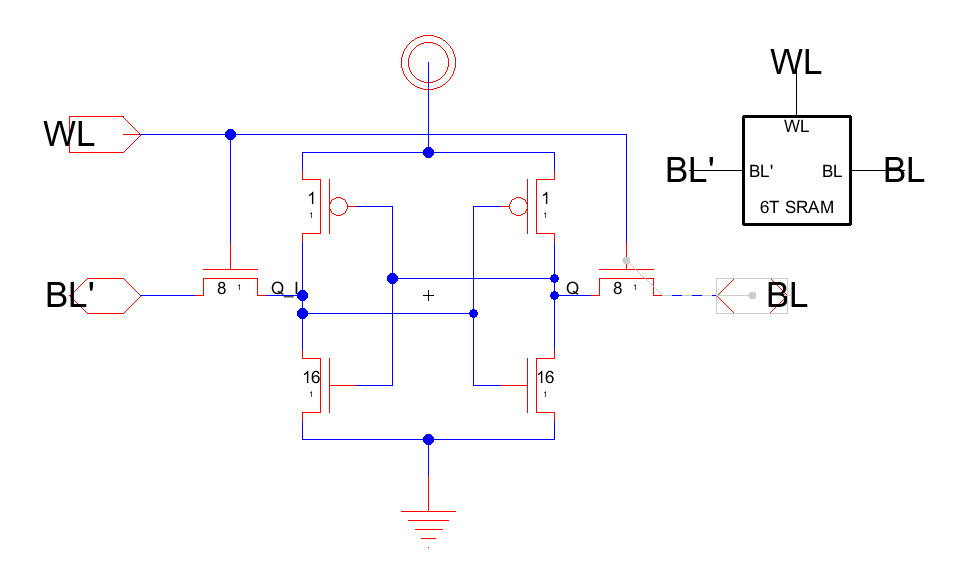
\includegraphics[width=1.0\textwidth]{Schematics/sram_cell_schematic.PNG}
  \caption{SRAM cell schematic}
  \label{fig:sram_cell_schematic}
\end{figure}

\subsection*{Control Block}
\begin{figure}[H]
  \centering
    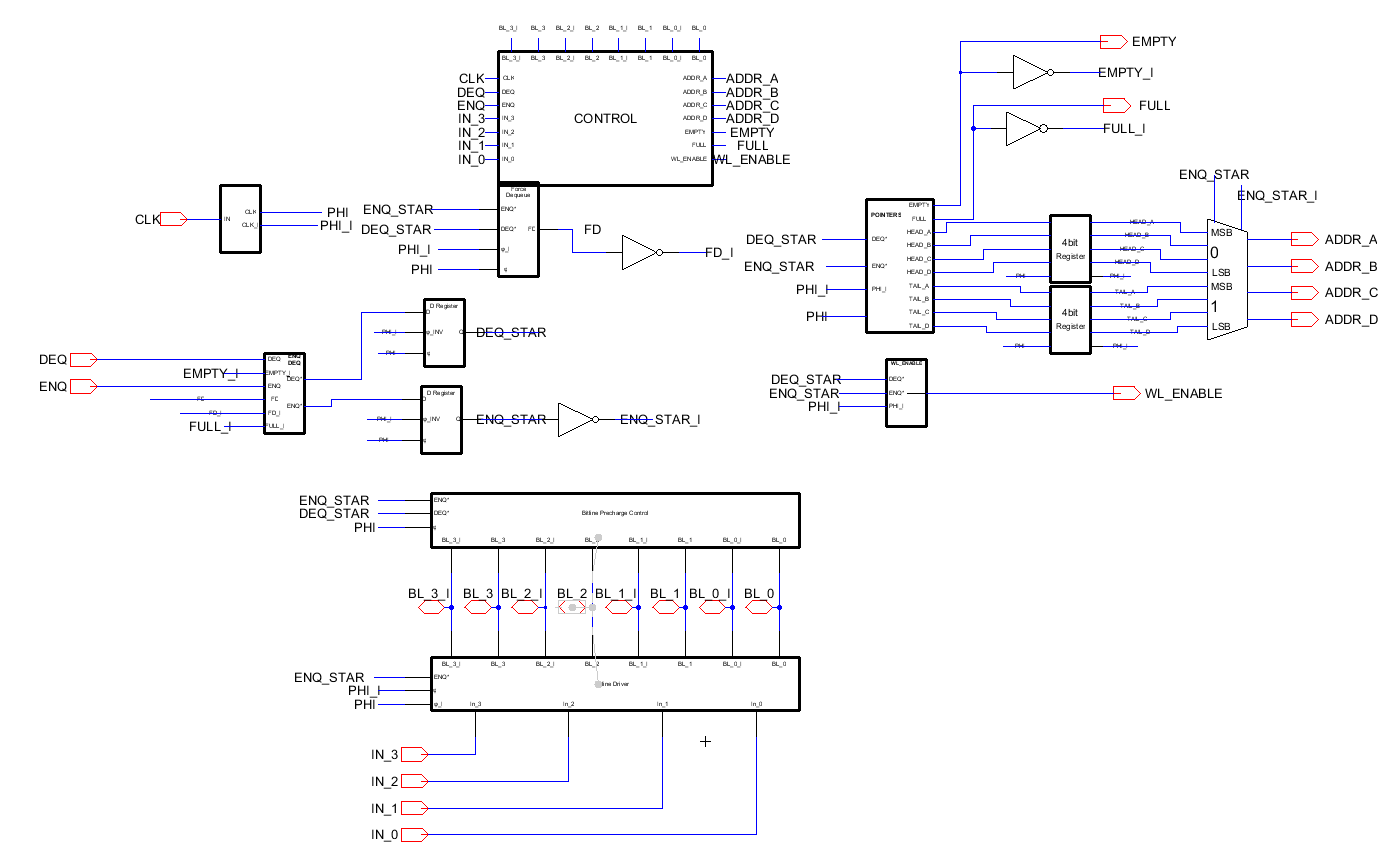
\includegraphics[width=1.0\textwidth]{Schematics/control_block_schematic.PNG}
  \caption{Control block toplevel schematic}
  \label{fig:control_block_schematic}
\end{figure}
\begin{figure}[H]
  \centering
    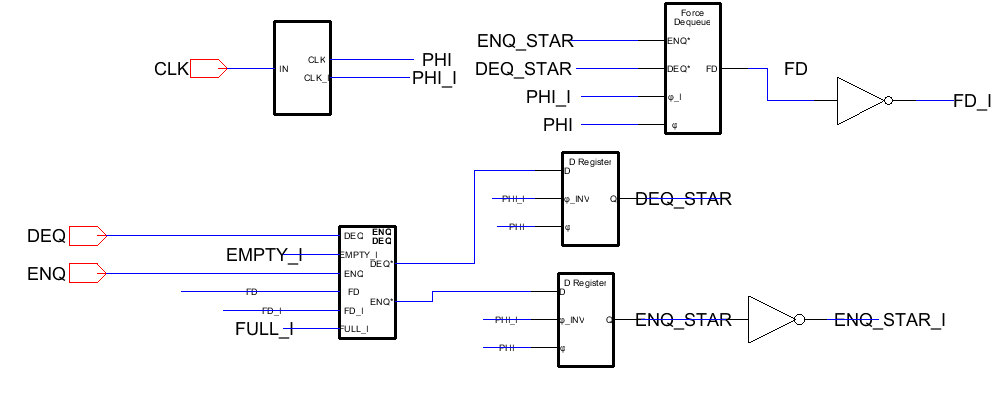
\includegraphics[width=1.0\textwidth]{Schematics/control_block_fd_clockgen_enqstar_deqstar_schematic.PNG}
  \caption{Control block schematic in detail, FD, clock generator, and ENQ*/DEQ* generation}
  \label{fig:control_block_fd_clockgen_enqstar_deqstar_schematic}
\end{figure}
\begin{figure}[H]
  \centering
    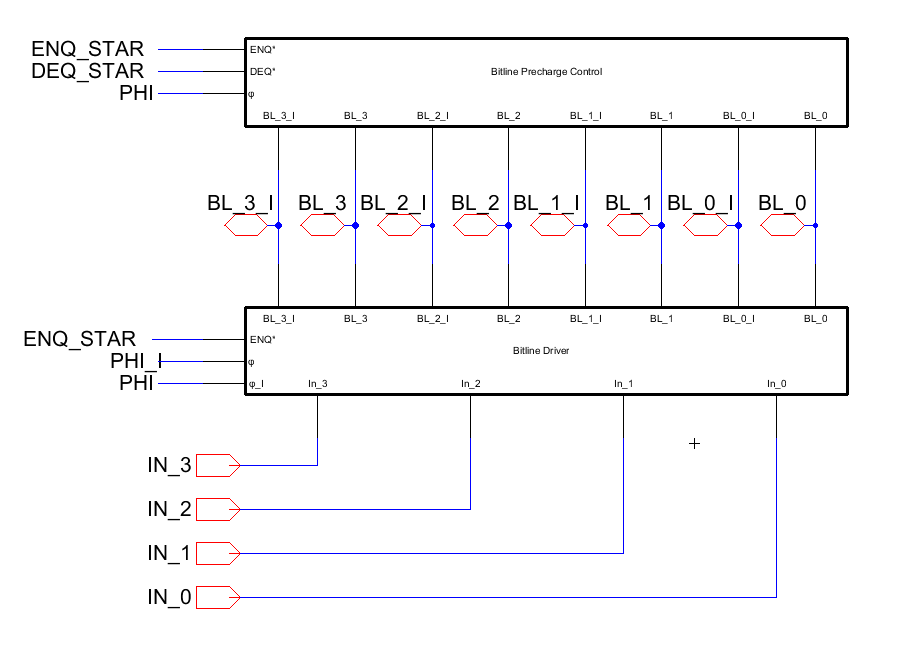
\includegraphics[width=1.0\textwidth]{Schematics/control_block_bitlinedriver_precharger_schematic.PNG}
  \caption{Control block schematic in detail, bitline driver and precharger}
  \label{fig:control_block_bitlinedriver_precharger_schematic}
\end{figure}
\begin{figure}[H]
  \centering
    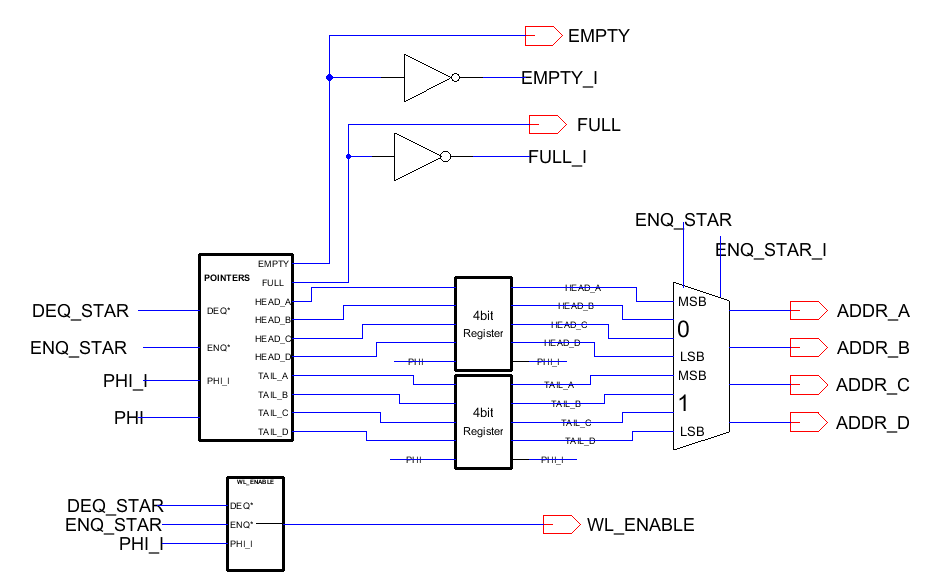
\includegraphics[width=1.0\textwidth]{Schematics/control_block_pointers_wlen_addrmux_emptyfull_schematic.PNG}
  \caption{Control block schematic in detail, pointers, WL\_EN, and EMPTY/FULL generation}
  \label{fig:control_block_pointers_wlen_addrmux_emptyfull_schematic}
\end{figure}

\subsection*{Clock Generator}
\begin{figure}[H]
  \centering
    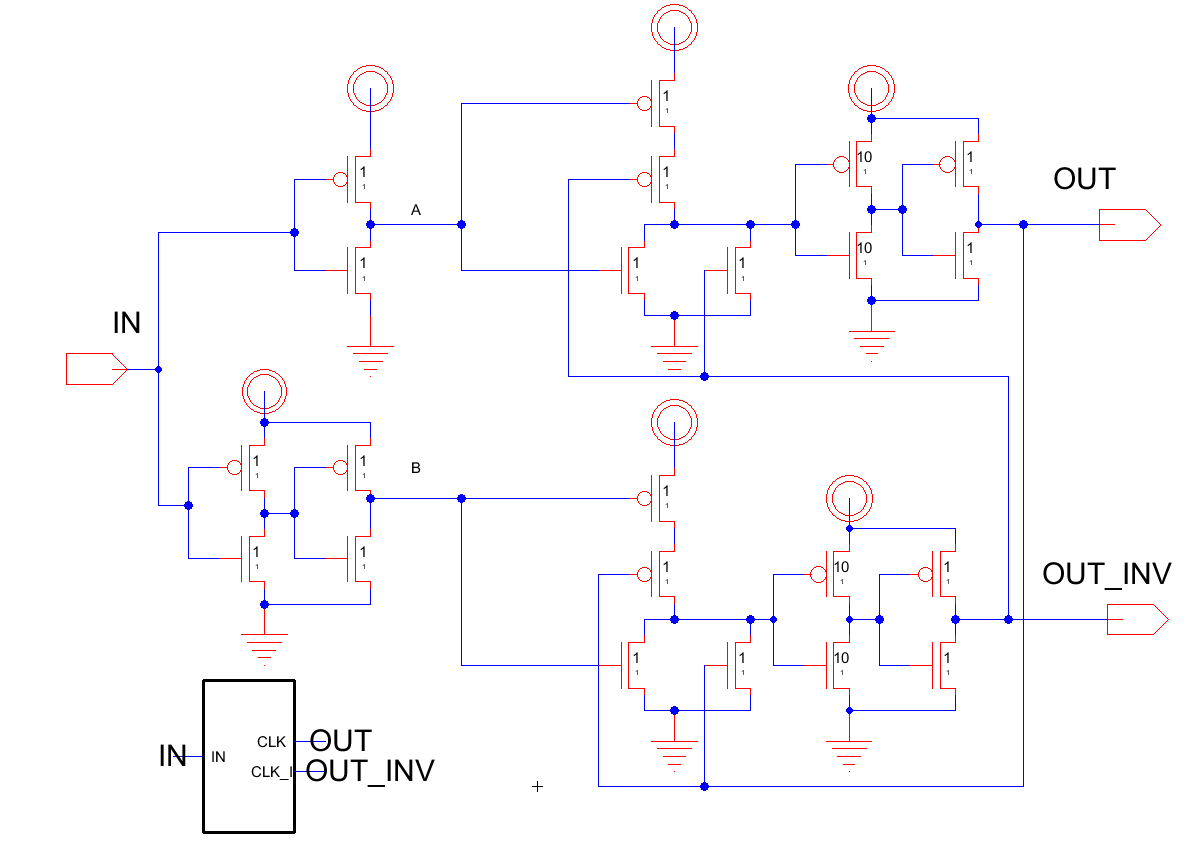
\includegraphics[width=1.0\textwidth]{Schematics/clk_gen_schematic.PNG}
  \caption{Clock generator schematic}
  \label{fig:clk_gen_schematic}
\end{figure}

\subsection*{Force Dequeue (FD)}
\begin{figure}[H]
  \centering
    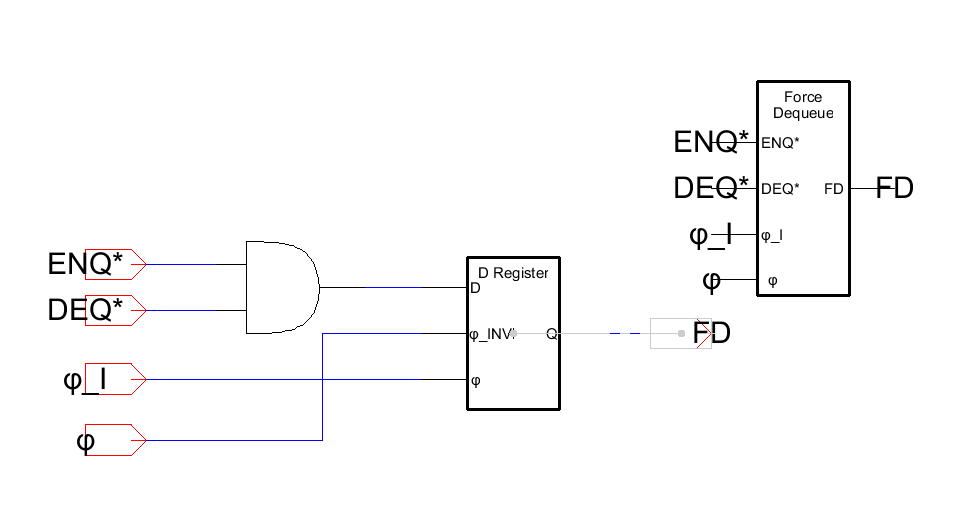
\includegraphics[width=1.0\textwidth]{Schematics/force_dequeue_schematic.PNG}
  \caption{Force dequeue generation schematic}
  \label{fig:force_dequeue_schematic}
\end{figure}

\subsection*{Pointers}
\begin{figure}[H]
  \centering
    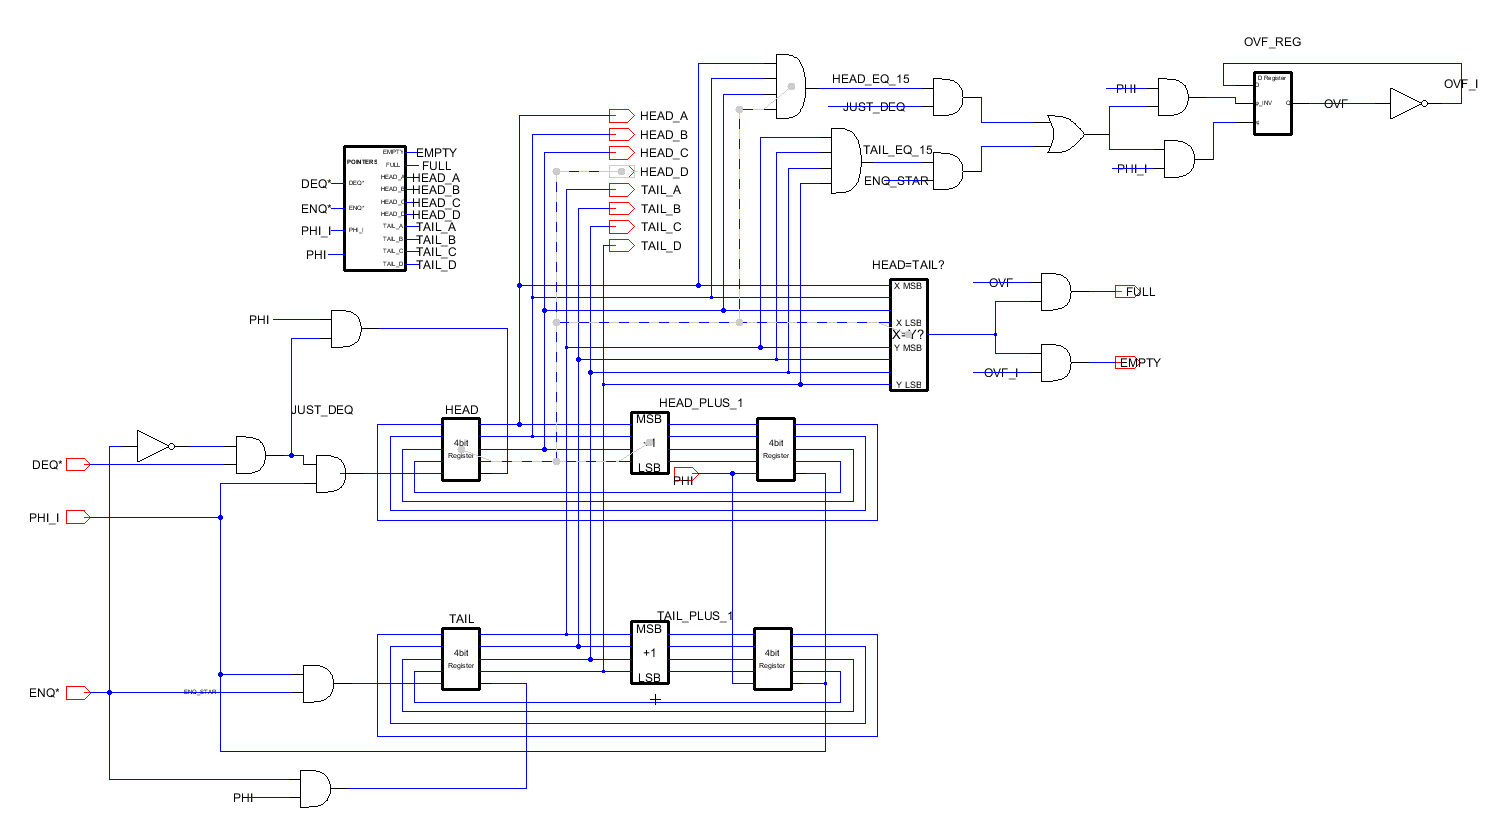
\includegraphics[width=1.0\textwidth]{Schematics/pointers_schematic.PNG}
  \caption{Pointers toplevel schematic}
  \label{fig:pointers_schematic}
\end{figure}
\begin{figure}[H]
  \centering
    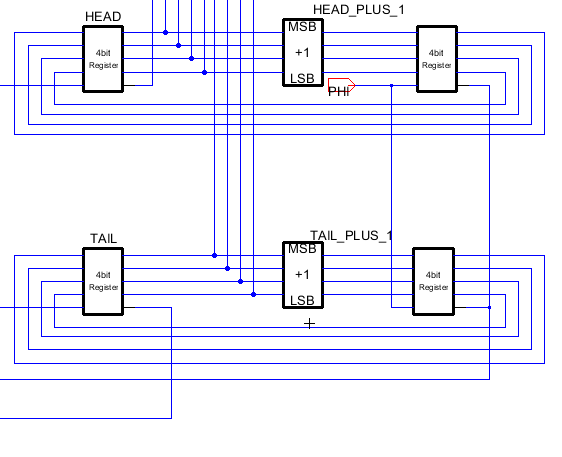
\includegraphics[width=1.0\textwidth]{Schematics/pointers_head_tail_state_schematic.PNG}
  \caption{Pointers schematic in detail, head/tail state}
  \label{fig:pointers_head_tail_state_schematic}
\end{figure}
\begin{figure}[H]
  \centering
    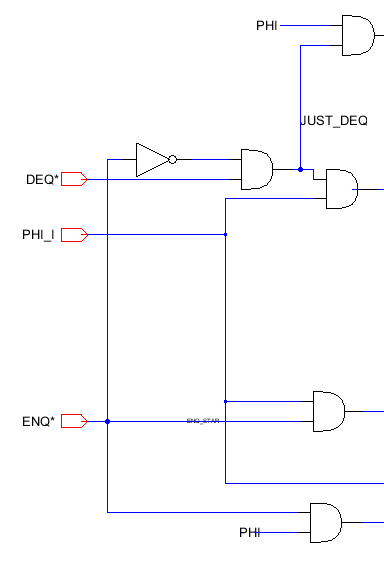
\includegraphics[width=1.0\textwidth]{Schematics/pointers_inputs_schematic.PNG}
  \caption{Pointers schematic in detail, inputs}
  \label{fig:pointers_inputs_schematic}
\end{figure}
\begin{figure}[H]
  \centering
    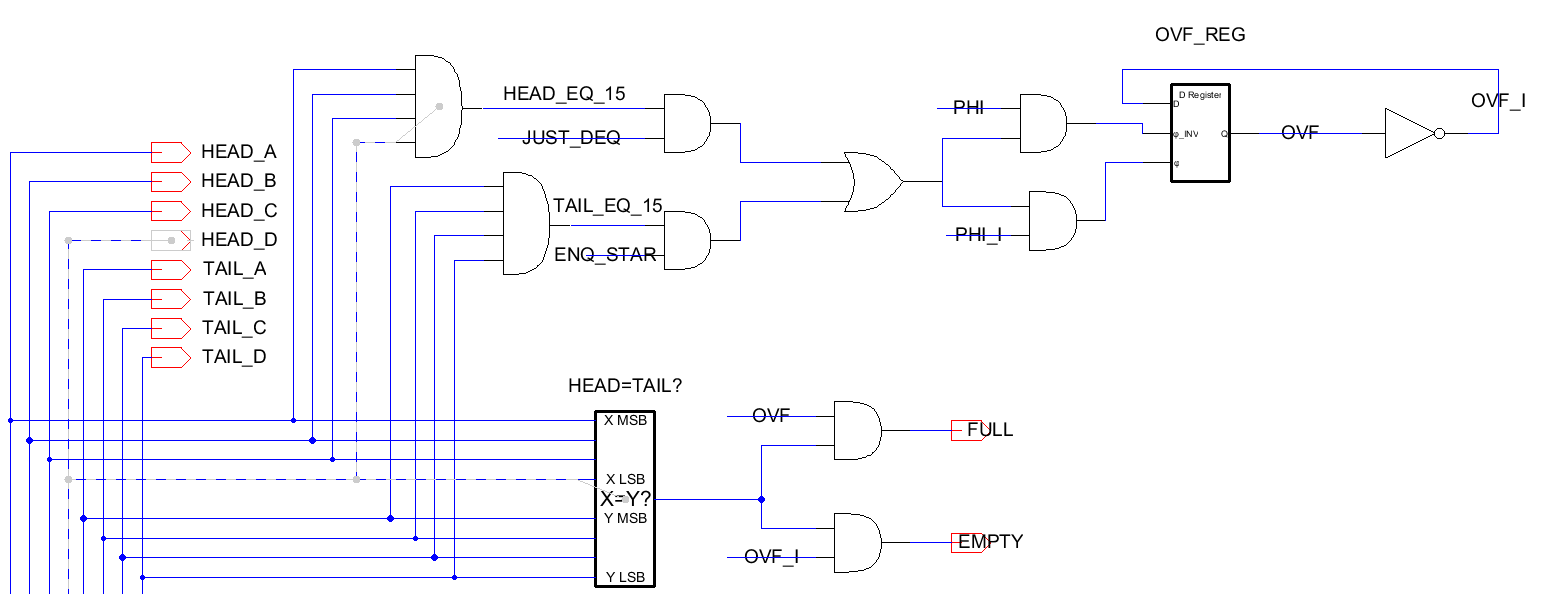
\includegraphics[width=1.0\textwidth]{Schematics/pointers_overflow_schematic.PNG}
  \caption{Pointers schematic in detail, overflow handler}
  \label{fig:pointers_overflow_schematic}
\end{figure}

\subsection*{D Latch}
\begin{figure}[H]
  \centering
    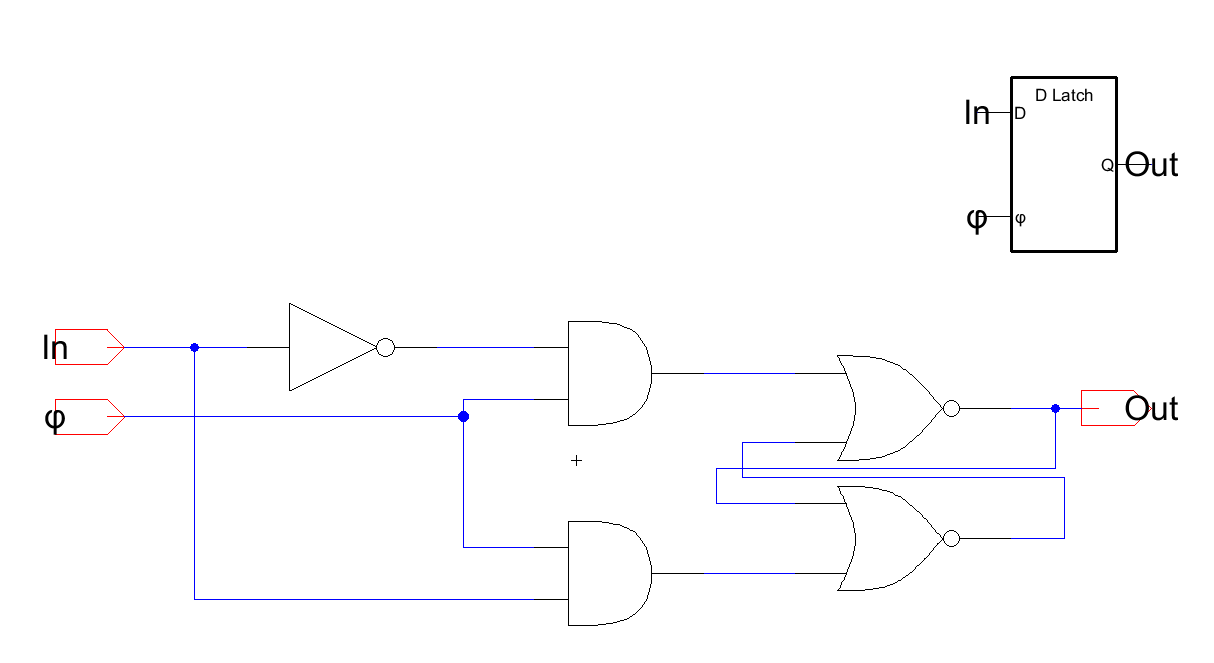
\includegraphics[width=1.0\textwidth]{Schematics/d_latch_schematic.PNG}
  \caption{D latch schematic}
  \label{fig:d_latch_schematic}
\end{figure}

\subsection*{D Register}
\begin{figure}[H]
  \centering
    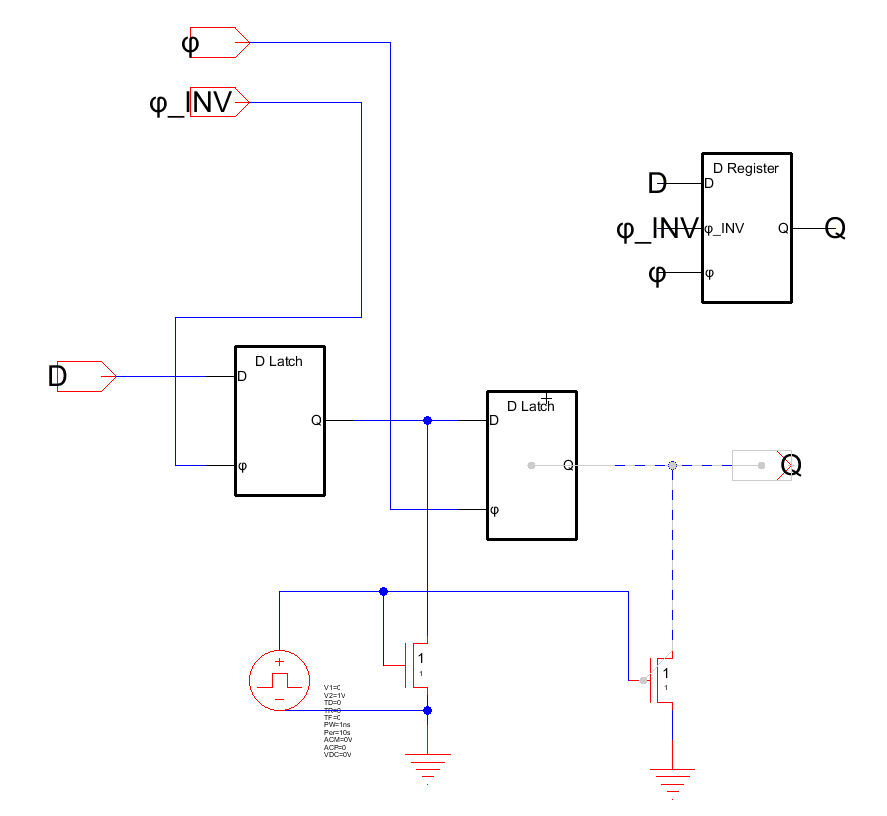
\includegraphics[width=1.0\textwidth]{Schematics/d_register_schematic.PNG}
  \caption{D register schematic}
  \label{fig:d_register_schematic}
\end{figure}

\subsection*{4-bit Register}
\begin{figure}[H]
  \centering
    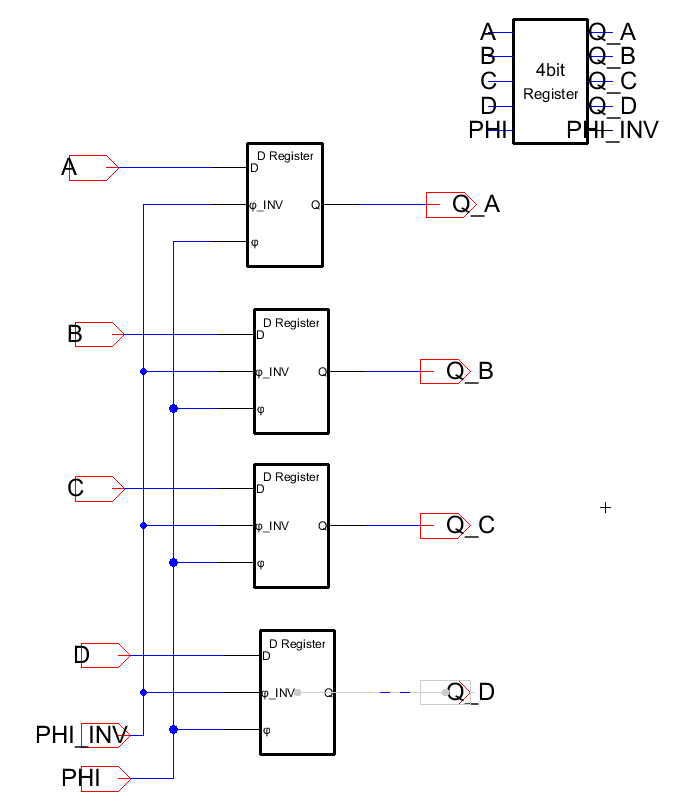
\includegraphics[width=1.0\textwidth]{Schematics/4_bit_register_schematic.PNG}
  \caption{4-bit register schematic}
  \label{fig:4_bit_register_schematic}
\end{figure}

\subsection*{Incrementer}
\begin{figure}[H]
  \centering
    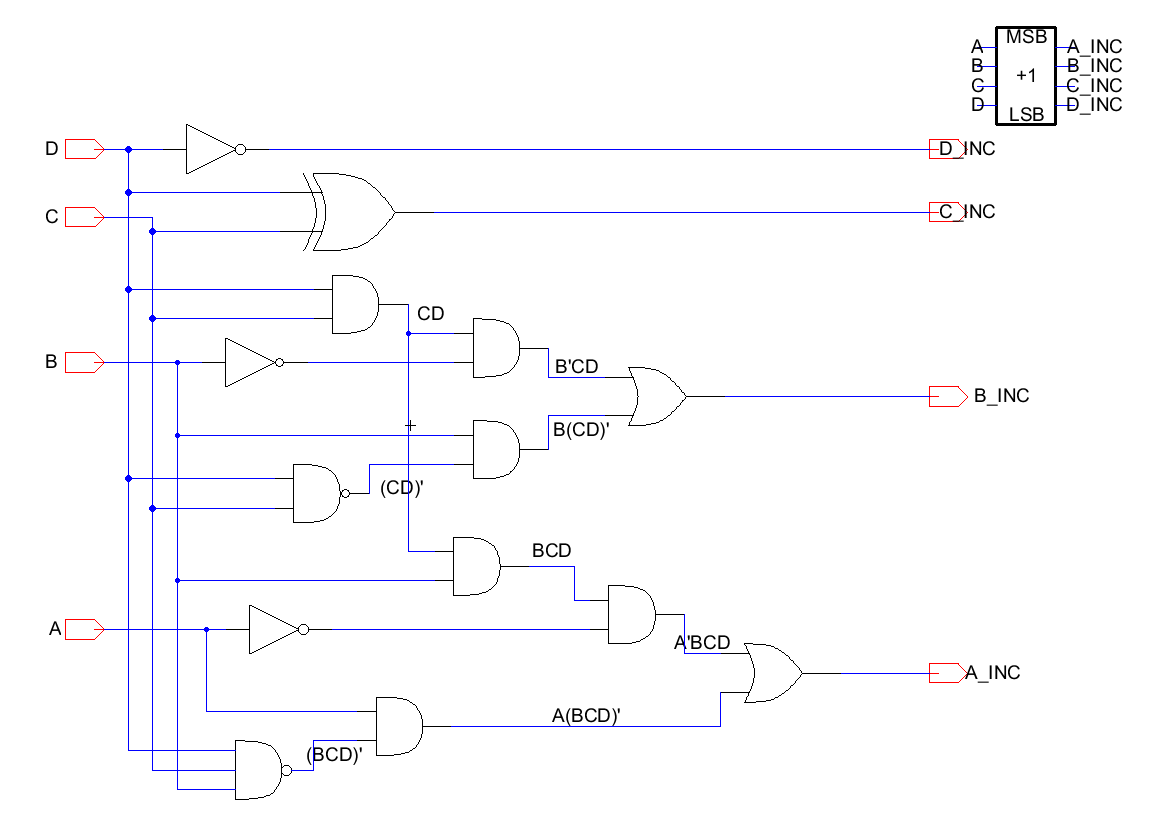
\includegraphics[width=1.0\textwidth]{Schematics/incrementer_schematic.PNG}
  \caption{Incrementer schematic}
  \label{fig:incrementer_schematic}
\end{figure}

\subsection*{Comparator}
\begin{figure}[H]
  \centering
    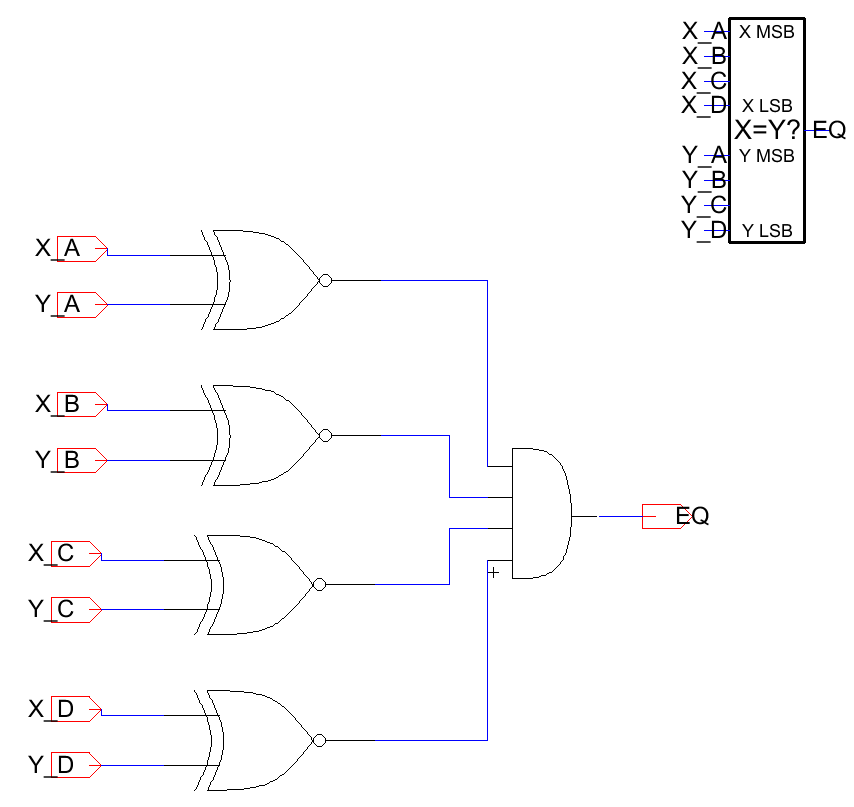
\includegraphics[width=1.0\textwidth]{Schematics/comparator_schematic.PNG}
  \caption{Equality comparator schematic}
  \label{fig:comparator_schematic}
\end{figure}

\subsection*{Mux}
\begin{figure}[H]
  \centering
    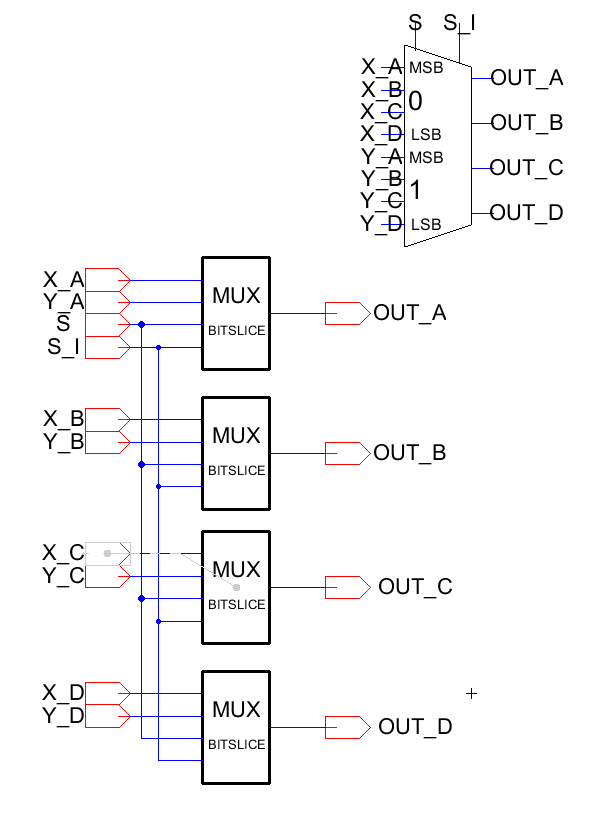
\includegraphics[width=1.0\textwidth]{Schematics/mux_schematic.PNG}
  \caption{Mux schematic}
  \label{fig:mux_schematic}
\end{figure}

\subsection*{Mux Bitslice}
\begin{figure}[H]
  \centering
    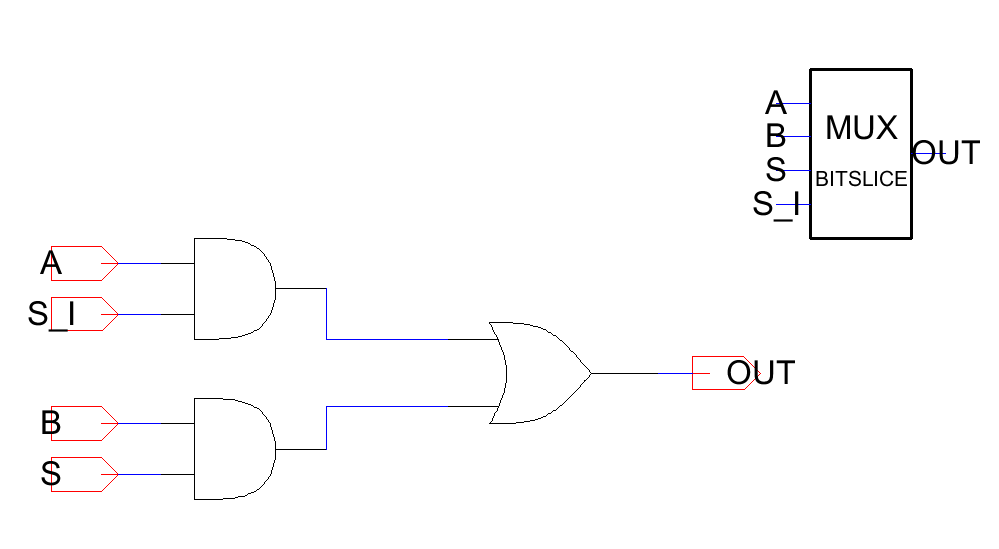
\includegraphics[width=1.0\textwidth]{Schematics/mux_bitslice_schematic.PNG}
  \caption{Mux bitslice schematic}
  \label{fig:mux_bitslice_schematic}
\end{figure}

\subsection*{Wordline Enable (WL\_EN)}
\begin{figure}[H]
  \centering
    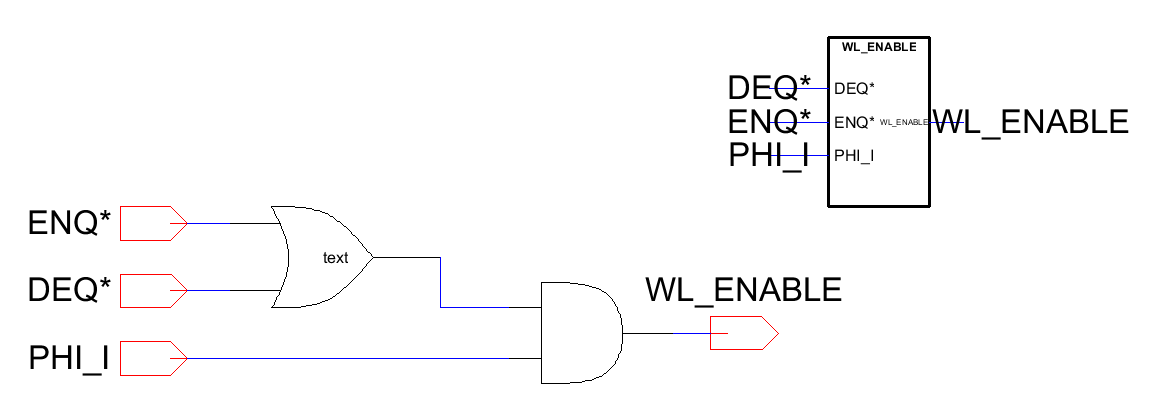
\includegraphics[width=1.0\textwidth]{Schematics/wl_enable_schematic.PNG}
  \caption{Word line enable generator schematic}
  \label{fig:wl_enable_schematic}
\end{figure}

\subsection*{ENQ*/DEQ* Generator}
\begin{figure}[H]
  \centering
    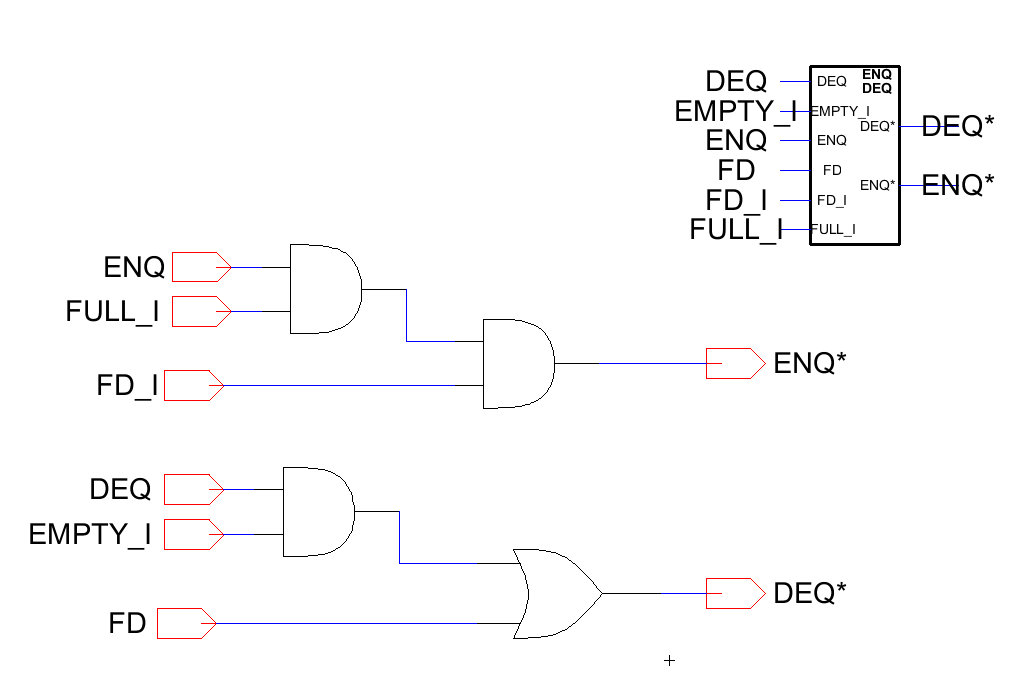
\includegraphics[width=1.0\textwidth]{Schematics/enqueue_dequeue_schematic.PNG}
  \caption{ENQ*/DEQ* generator schematic}
  \label{fig:enqueue_dequeue_schematic}
\end{figure}

\subsection*{4-bit Bitline Precharger}
\begin{figure}[H]
  \centering
    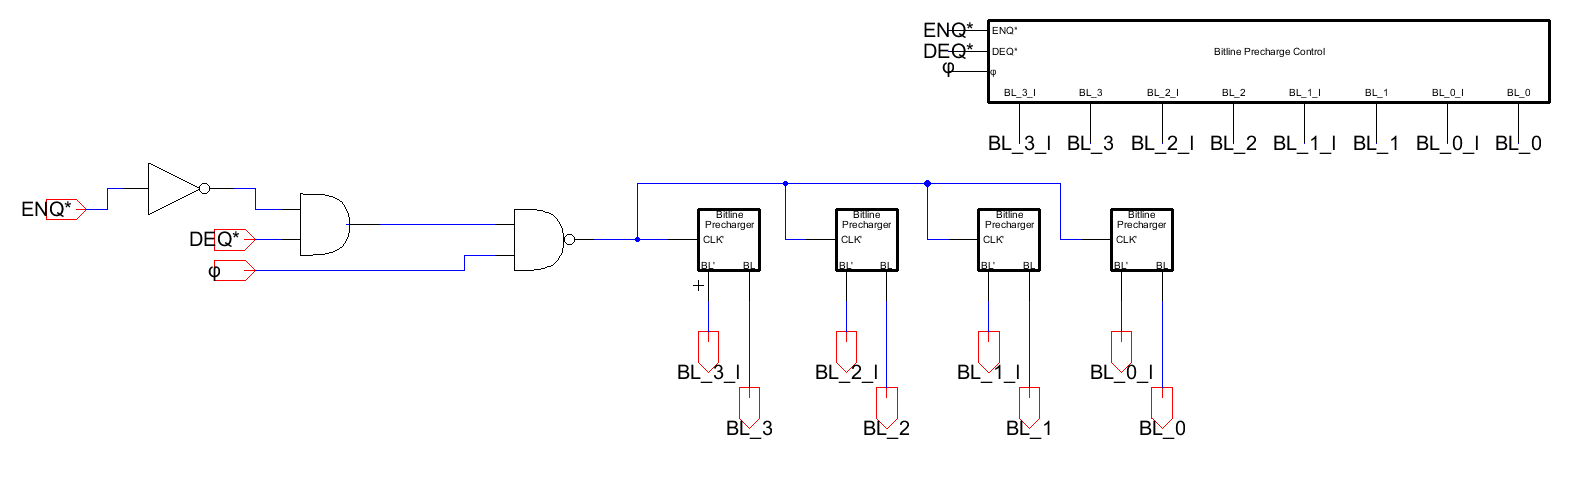
\includegraphics[width=1.0\textwidth]{Schematics/4_bit_precharge_schematic.PNG}
  \caption{4-bit bitline precharger schematic}
  \label{fig:4_bit_precharge_schematic}
\end{figure}

\subsection*{1-bit Bitline Precharger}
\begin{figure}[H]
  \centering
    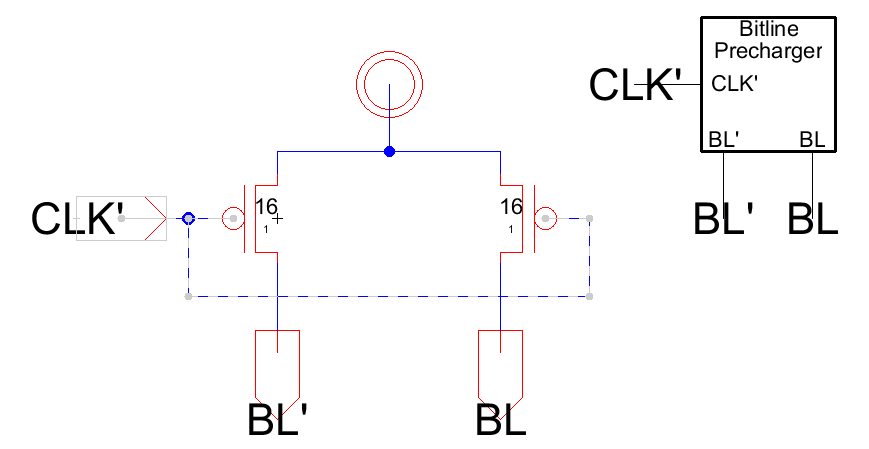
\includegraphics[width=1.0\textwidth]{Schematics/precharge_schematic.PNG}
  \caption{1-bit bitline precharger schematic}
  \label{fig:precharge}
\end{figure}

\subsection*{Bitline Driver}
\begin{figure}[H]
  \centering
    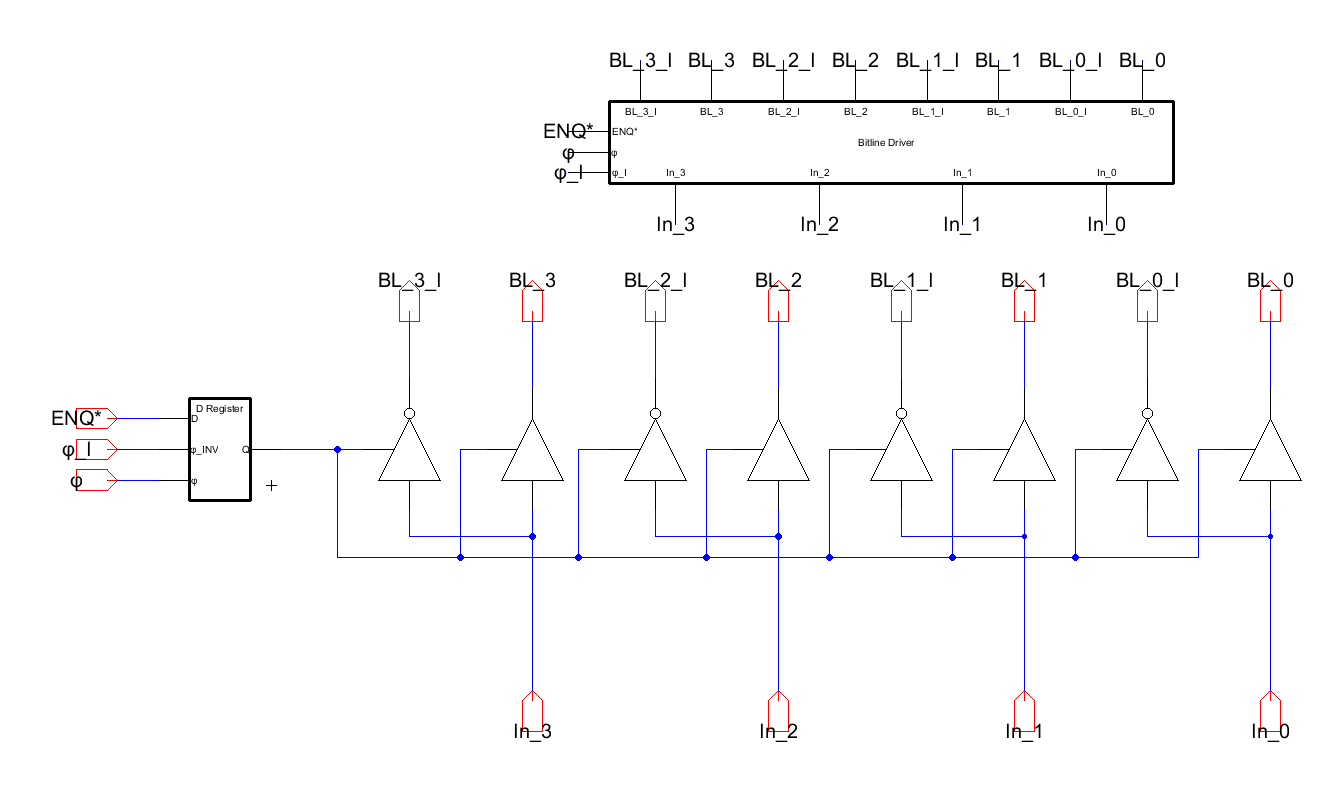
\includegraphics[width=1.0\textwidth]{Schematics/bitline_driver_schematic.PNG}
  \caption{Bitline driver schematic}
  \label{fig:bitline_driver_schematic}
\end{figure}

\subsection*{Inverter}
\begin{figure}[H]
  \centering
    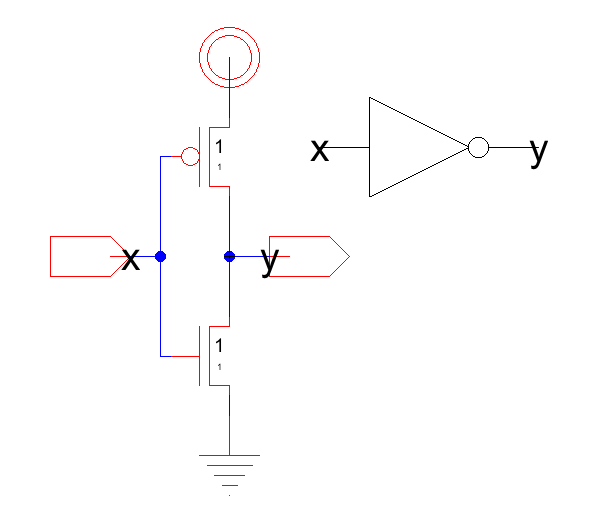
\includegraphics[width=1.0\textwidth]{Schematics/inverter_schematic.PNG}
  \caption{Inverter schematic}
  \label{fig:inverter_schematic}
\end{figure}

\subsection*{NAND2}
\begin{figure}[H]
  \centering
    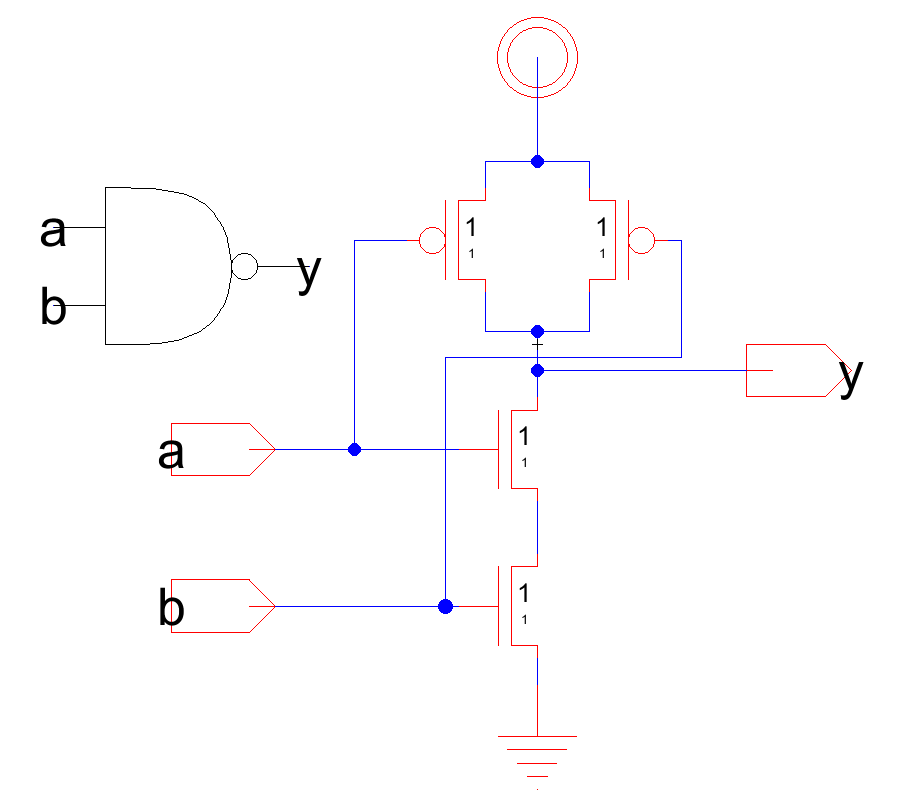
\includegraphics[width=1.0\textwidth]{Schematics/nand_gate_schematic.PNG}
  \caption{NAND2 gate schematic}
  \label{fig:nand_gate_schematic}
\end{figure}

\subsection*{AND2}
\begin{figure}[H]
  \centering
    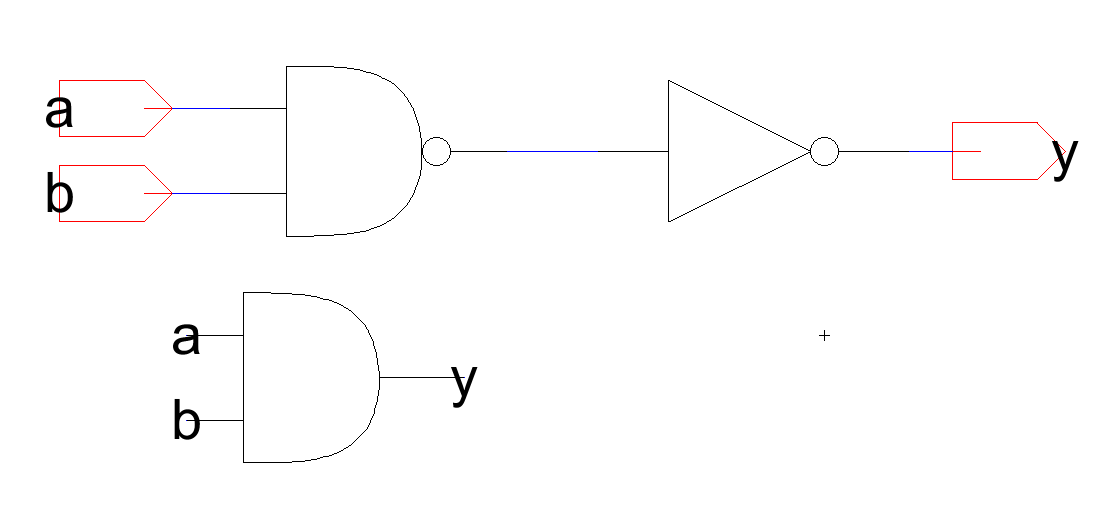
\includegraphics[width=1.0\textwidth]{Schematics/and_gate_schematic.PNG}
  \caption{AND2 gate schematic}
  \label{fig:and_gate_schematic}
\end{figure}

\subsection*{AND4}
\begin{figure}[H]
  \centering
    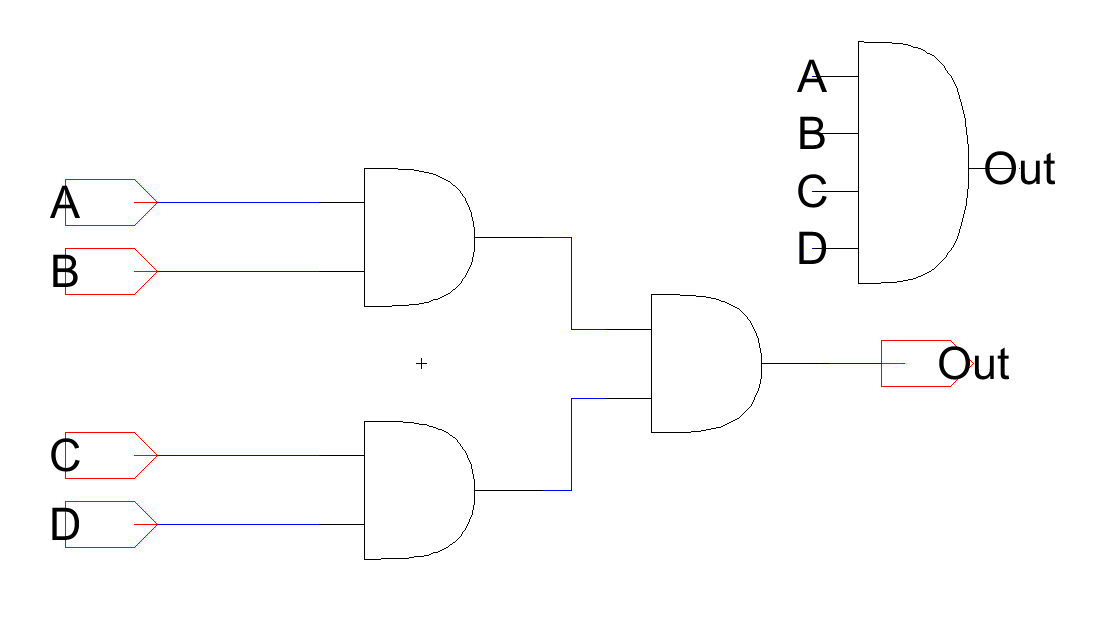
\includegraphics[width=1.0\textwidth]{Schematics/and4_gate_schematic.PNG}
  \caption{AND4 gate schematic}
  \label{fig:and4_gate_schematic}
\end{figure}

\subsection*{NOR2}
\begin{figure}[H]
  \centering
    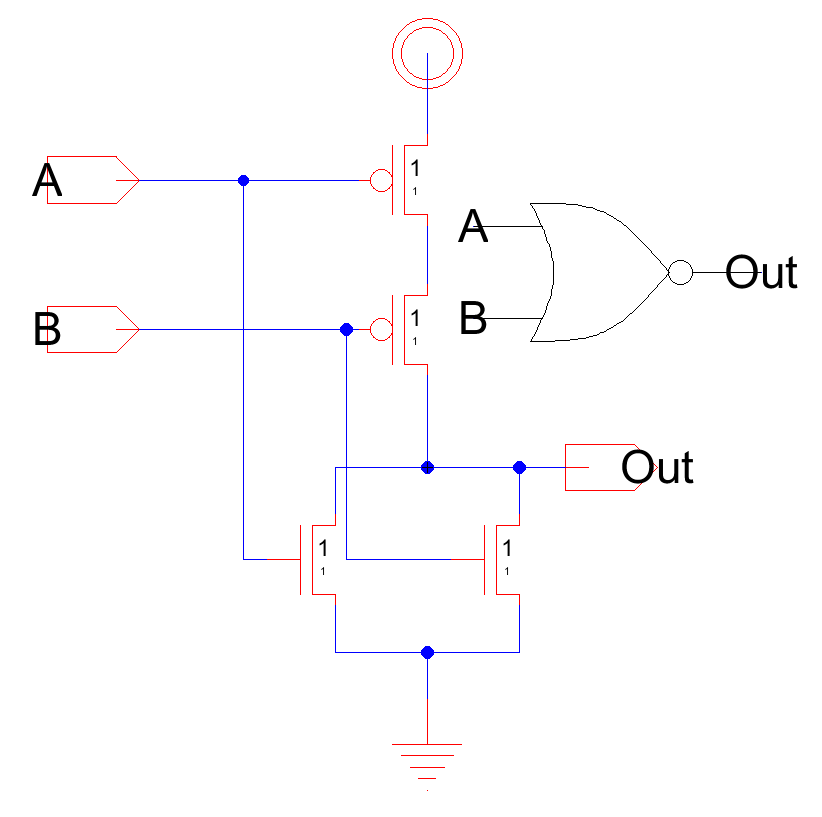
\includegraphics[width=1.0\textwidth]{Schematics/nor_gate_schematic.PNG}
  \caption{NOR2 gate schematic}
  \label{fig:nor_gate_schematic}
\end{figure}

\subsection*{Decoder}
\begin{figure}[H]
  \centering
    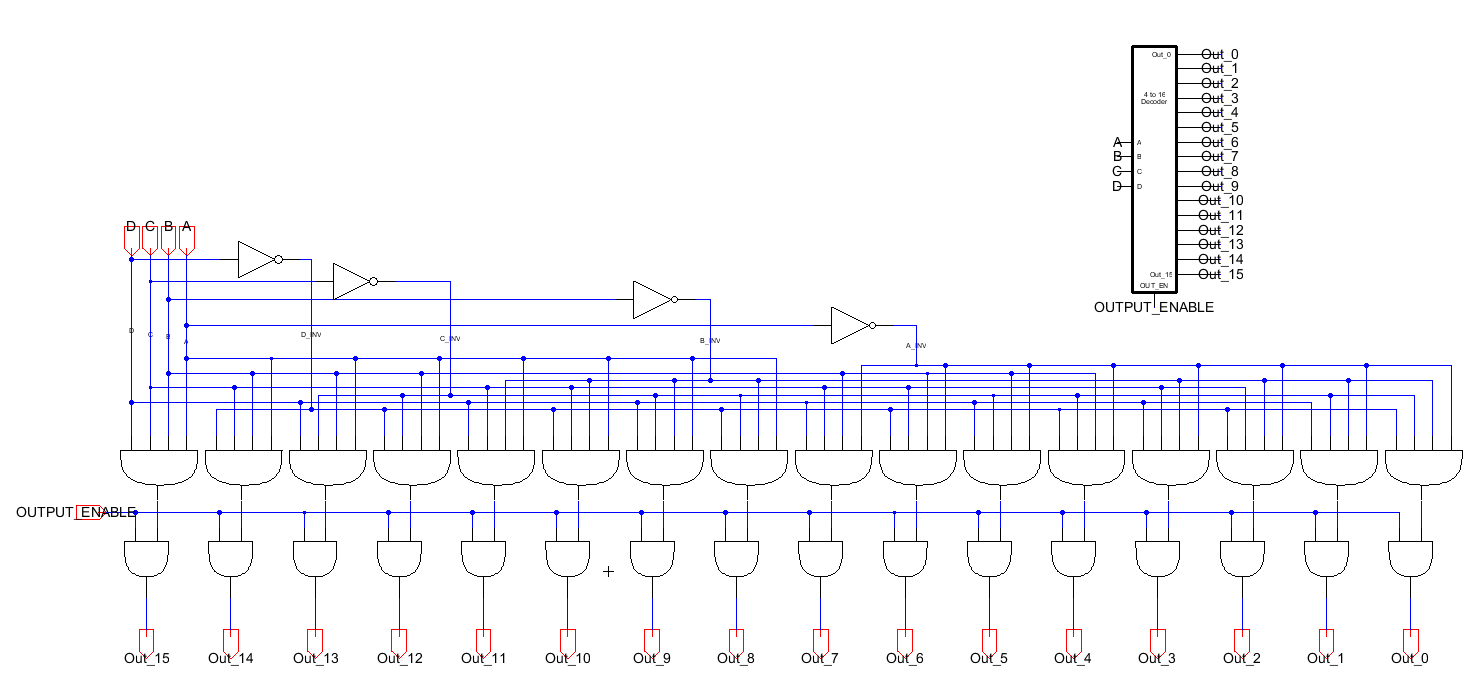
\includegraphics[width=1.0\textwidth]{Schematics/decoder_schematic.PNG}
  \caption{4-to-16 decoder schematic}
  \label{fig:decoder_schematic}
\end{figure}

\subsection*{Tri-State Buffer}
\begin{figure}[H]
  \centering
    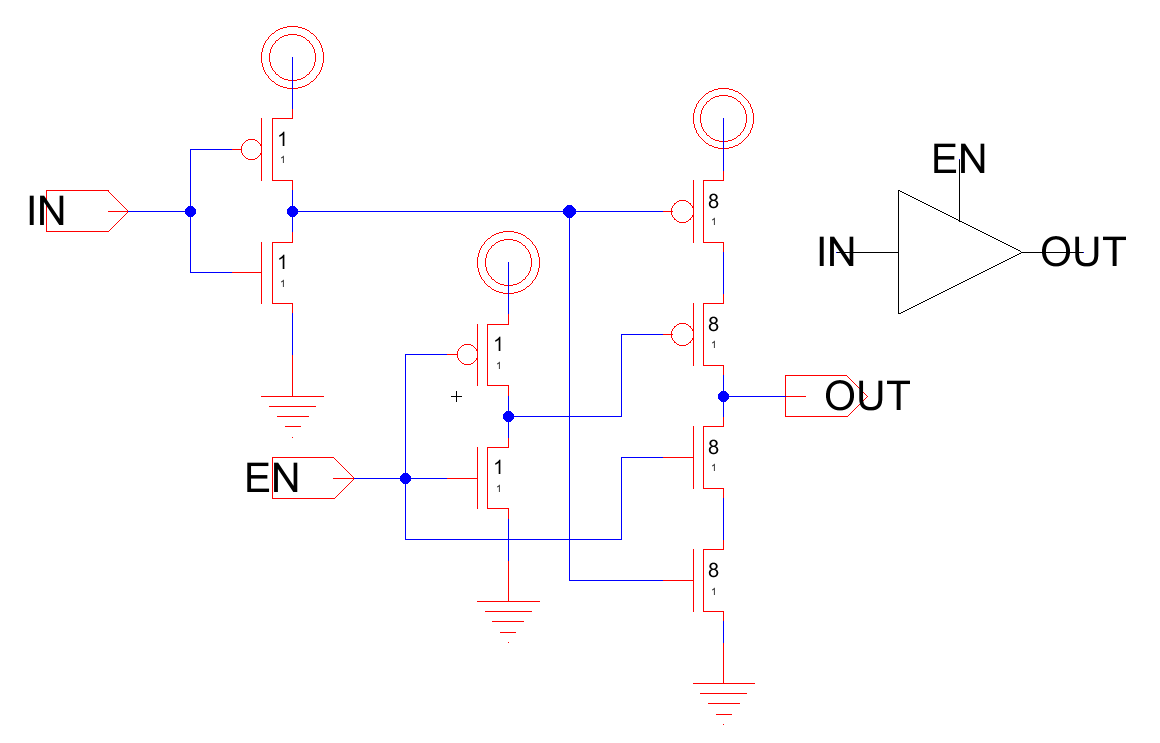
\includegraphics[width=1.0\textwidth]{Schematics/tristate_buffer_schematic.PNG}
  \caption{Tri-state buffer schematic}
  \label{fig:tristate_buffer_schematic}
\end{figure}

\subsection*{Tri-State Inverter}
\begin{figure}[H]
  \centering
    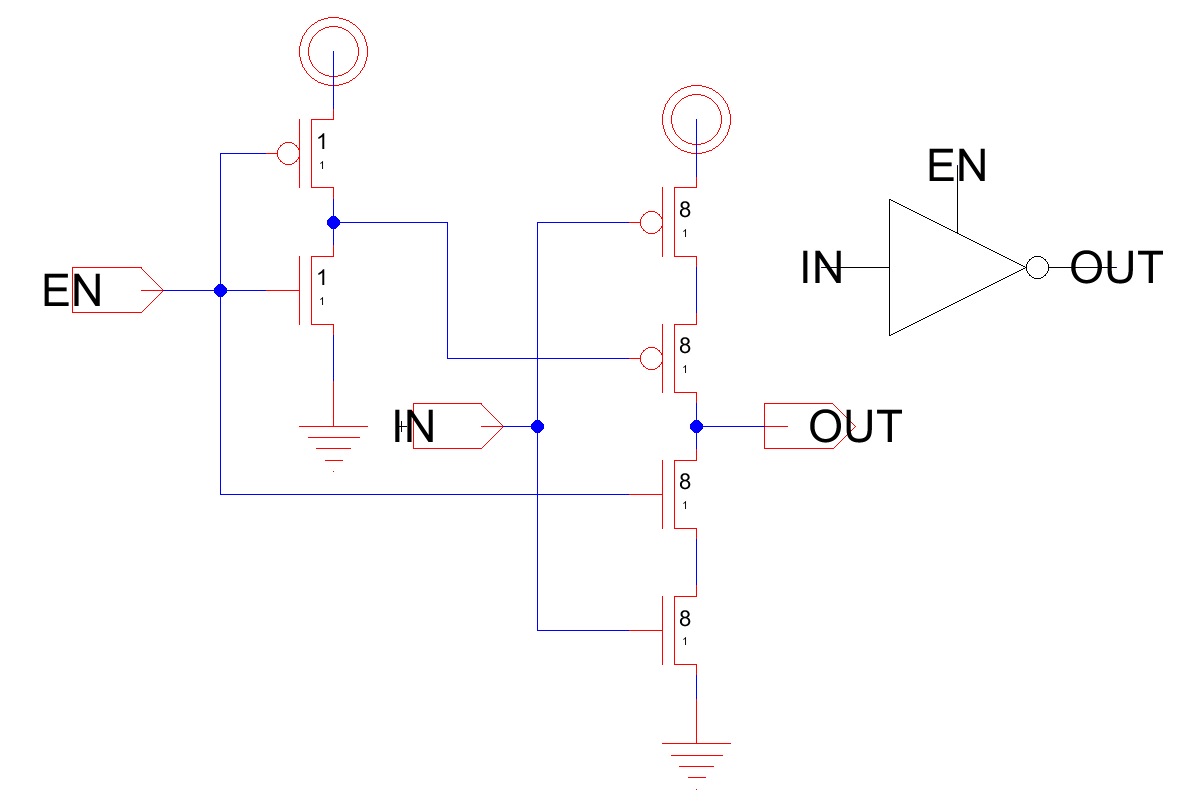
\includegraphics[width=1.0\textwidth]{Schematics/tristate_inverter_schematic.PNG}
  \caption{Tri-state inverter schematic}
  \label{fig:tristate_inverter_schematic}
\end{figure}

\newpage
\section*{Timing of Key Signals}

\newpage
\section*{Memory Operation and Design Choices}
\subsection*{Control Block}
The control block is broken down as follows;
\begin{enumerate}

  \item Clock Generator

  The clock generator is used to generate non-overlapping waveforms for the inputs to the D registers. This is needed because these registers consist of two D-latches wired in series. If the two clocks overlapped, the second D latch would sample the input at the same time as the first, meaning that the output woudn't update on the edge of a clock cycle, as it should be.

  \item Force Dequeue

  This module is designed to trigger a dequeue (following an enqueue) when both Enqueue and Dequeue are asserted by the user. It consists of a D register that latches the state of (ENQ* and DEQ*) on the falling edge of $\phi$, or the rising edge of $\phi'$.

  \item ENQ*/DEQ* Generator

  This module generates two internal signals, ENQ* and DEQ*, that are used to trigger an enqueue or a dequeue, respectively. ENQ* is set whenever Enqueue is asserted by the user, the queue is not full, and a dequeue is not forced. (It will only trigger when a dequeue is not forced to prevent the user from enqueueing in the clock cycle following a simultaneous enqueue and dequeue, since this clock cycle is when the dequeue will occur.) DEQ* is set whenever the user asserts Dequeue and the queue is not empty, or when a dequeue from a simultaneous enqueue/dequeue event needs to be completed.

  The ENQ* and DEQ* outputs from this module are fed into registers to latch the values until the next clock cycle. The user therefore does not have to assert Enqueue and Dequeue for the entire clock cycle.

  \item WL Enable

  Whenever ENQ* or DEQ* are high, the WL Enable module enables and disables the decoder output in the memory cell, which determines which word line is being set high. (See Decoder for more information on why an enable input was necessary.)

  \item Pointers

  The Pointers module holds the state for the head and tail pointers and contains the logic for updating these pointers and determining if the queue is empty or full. It is broken down as follows:
  \begin{enumerate}
    \item Head (HEAD) and Tail (TAIL) Pointers

    These contain the addresses of where the queue will enqueue to/dequeue from the next time Enqueue or Dequeue are triggered. In our queue, enqueues add elements to the tail, and dequeues remove elements from the head. Therefore, the address of tail is always greater than the address of head.

    HEAD is incremented whenever DEQ* is high, ENQ* is not high, and a falling edge of the clock occurs. Likewise, TAIL is incremented whenever ENQ* is high, DEQ* is not high, and a falling edge of the clock occurs.

    \item Head and Tail Incrementers (HEAD\_PLUS\_1 and TAIL\_PLUS\_1)

    These are combinational circuits that increment the current values of HEAD and TAIL. They are used to increment the current values of HEAD and TAIL on enqueues and dequeues, respectively.

    The incremented values are followed by registers that toggle on the rising edge of the clock in order to prevent these incremented values from arriving too early at HEAD/TAIL and updating HEAD/TAIL prematurely. Without them, we ran into an issue where HEAD and TAIL would sometimes "jump" to higher values, even though they were supposed to rise by 1.

    \item Comparator (HEAD = TAIL)

    This comparator is a combinational circuit that checks whether the values of HEAD and TAIL are equal to each other. It outputs whether the queue is full (FULL) or empty (EMPTY) depending on whether OVF has been set by OVF\_REG (see below).

    \item OVF\_REG

    This portion of the circuit checks when the current values of HEAD and TAIL are equal to 15, signalling that they are about to wrap-around to address 0. When this happens, OVF\_REG is toggled. (Observe that OVF\_REG is always set high when TAIL wraps around and is always set low when HEAD wraps around. This is because OVF\_REG starts at 0, TAIL wraps around first (it's ahead of HEAD), and TAIL wrapping around is always followed by HEAD wrapping around (and vice-versa).)

    Also observe that when OVF is set and HEAD == TAIL, then the queue is full since TAIL has wrapped around and HEAD has not yet. Likewise, when OVF is not set and HEAD == TAIL, the queue is empty since HEAD has wrapped around and TAIL has not yet. (See above for more information on the Comparator.)
  \end{enumerate}

  The HEAD and TAIL outputs of Pointers are fed into two 4-bit registers that latch on the rising edge of the clock, and the outputs of these registers are muxed to the address bits of the SRAM memory block. The outputs are latched to prevent the address bits from updating before an enqueue or dequeue is performed. They are muxed to update the address bits according to whether an enqueue or dequeue is performed. (For example, an enqueue will update the address lines to TAIL, while a dequeue will update them to HEAD.)

  \item Bitline Precharge Control

  This module triggers a precharge of the bitlines whenever ENQ* is low and DEQ* is high, and the clock is high. (The NAND gate is present instead of an AND because the precharge enable is active-low.)

  Each bit-level precharge circuit consists of two PMOS transistors sized at $W = 16$. We sized them like this to overcome the additional capacitance presented on the bitline by the 16 SRAM memory cells.

  \item Bitline Driver

  The bitline driver is used during enqueuing to write to the memory cells. Writes are triggered whenever ENQ* is asserted and on the rising edge of the clock cycle, and last for a full clock cycle.
\end{enumerate}

\subsection*{Memory Block}
The memory block is broken down as follows:
\begin{enumerate}
  \item 6T SRAM Cells

  There are 64 SRAM cells, each holding a single bit (16 words x 4 bits per word). These cells consist of four NMOS and two PMOS transistors arranged in a cross-coupled inverter configuration. (This is the same configuration presented in lecture).

  The two access transistors are sized at $W = 8$ in order to prevent the cell from being overwritten when the bitline changes suddenly. We originally had them at $W = 4$ when we tested the milestone, but when we tested the entire array, we found that when dequeueing (which involves precharging the bitlines), some cells were being overwritten.

  The bottom two NMOS transistors are sized at $W = 16$ to prevent read upsets - the value of $Q$ being overwritten when the cell is being read. Originally, for the milestone, they were set at $W = 8$, but we doubled the width to keep the ratio between this $W$ and $W{access}$ the same after we changed $W{access}$ to 8, as described above.

  \item Decoder

  This 4-to-16 decoder is used to reduce the amount of address lines needed from the control block. It is a standard CMOS decoder design that outputs the 16 possible minterms generated from 4 logic inputs (A, B, C, and D). It also includes an output enable bit to turn off the decoder's output when we are not reading or writing, therefore ensuring that the word line of one bit is not high at once. (If one word line was high at all times, we would be reading or writing at all times, which would interfere with reading or writing at the intended time because the bit lines would need to be precharged or driven.)
\end{enumerate}

\newpage
\section*{Optimization of Energy}
One of the ways in which we optimized the energy was by minimizing the number of transistors throughout the design. For example, in the 4-bit bitline precharge module, the individual bitline precharge modules require CLK to be asserted low in order for that bitline to be precharged, since the precharging is controlled by PMOS transistors. The logic function for precharging is that ENQ* is not asserted, DEQ* is, and the clock is high. We originally had it so that all of these values were being ANDed and then inverted, but we reduced this just to a NAND gate because the inverter was redundant. This reduces static energy usage slightly because there are two fewer transistors without the inverter.

Another way we reduced the energy was by keeping $V_{dd}$ low, at 0.8 V. We thought about increasing $V_{dd}$ to 1 V to reduce the delay, but we reasoned that this was unnecessary because delay was not a specification that we were specifically asked to optimize in this project. Increasing $V_{dd}$ also would lead to more static power dissipation (since $V_{dd}$ is higher), as well as potentially more dynamic power dissipation (since there would be a wider voltage range in which the two transistors in an inverter would be turned on at once).

We also minimized the amount of energy used by keeping transistors sized as reasonably small as possible. For example, in the 6T memory cell, we sized the transistors at the minimum size ($W = 16$) so that read upsets would be avoided and changes on the bit lines would not cause the stored values to be overwritten. (See description of bit cell circuit operation for more detail on why we had to do this.) We also kept all other transistors in the design minimum-sized, except for the bit-line drivers and prechargers (which were needed to overcome the bitline capacitance). Keeping $W$ small reduces the amount of static current drawn and thus reduces the amount of power used.

\newpage
\section*{Validation of Correctness}
We validated the correctness of the design by unit-testing each module, and then running integration tests on the whole queue.

\subsection*{Unit Tests}
The unit tests were done to ensure that each component operated according to the specifications given in our design above. Most of them do not require a description since many are combinational or simple sequeuntial circuits. If a description is needed, it is provided in the appropriate test.
\subsubsection*{Clock Generator}
\begin{figure}[H]
  \centering
    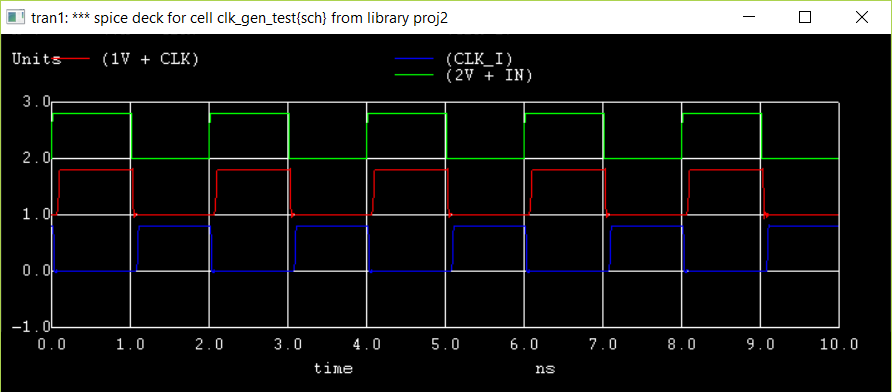
\includegraphics[width=1.0\textwidth]{clk_gen_test.PNG}
  \caption{Clock generator test}
  \label{fig:clk_gen_test}
\end{figure}
\begin{figure}[H]
  \centering
    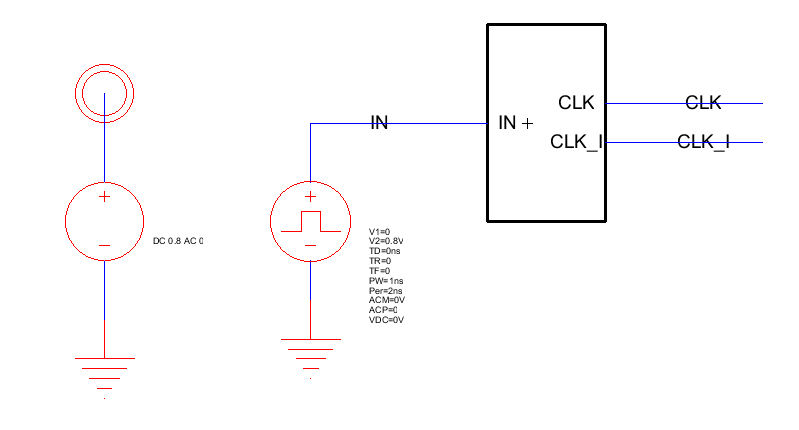
\includegraphics[width=1.0\textwidth]{TestSchematics/clk_gen.PNG}
  \caption{Clock generator test schematic}
\end{figure}

\subsubsection*{Comparator}
The comparator was broken into 3 tests: numbers the same, numbers were different but swapped, and numbers were different.
\begin{figure}[H]
  \centering
    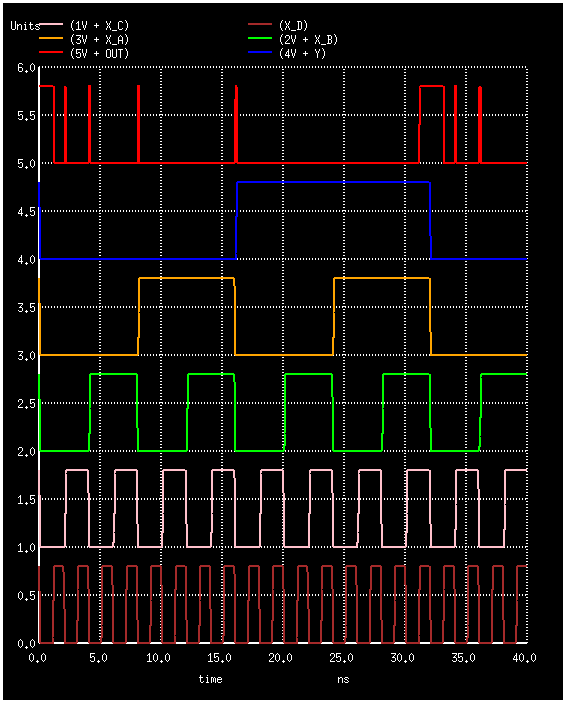
\includegraphics[width=1.0\textwidth]{comparator_test_diff.PNG}
  \caption{Comparator test, different}
  \label{fig:comparator_test_diff}
\end{figure}
\begin{figure}[H]
  \centering
    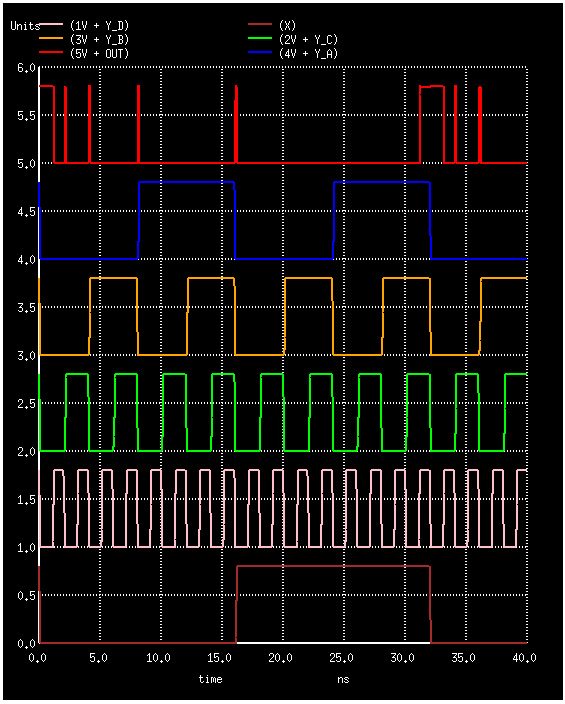
\includegraphics[width=1.0\textwidth]{comparator_test_diff_swapped.PNG}
  \caption{Comparator test, different and swapped}
  \label{fig:comparator_test_diff_swapped}
\end{figure}
\begin{figure}[H]
  \centering
    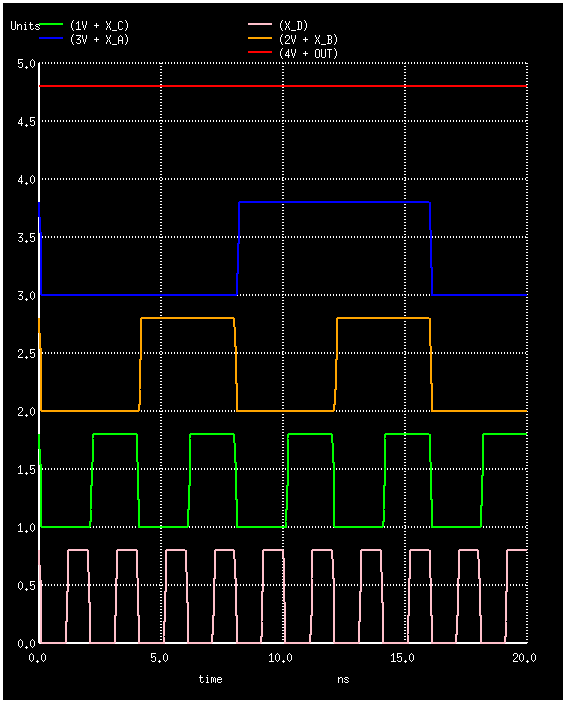
\includegraphics[width=1.0\textwidth]{comparator_test_same.PNG}
  \caption{Comparator test, same}
  \label{fig:comparator_test_same}
\end{figure}
\begin{figure}[H]
  \centering
    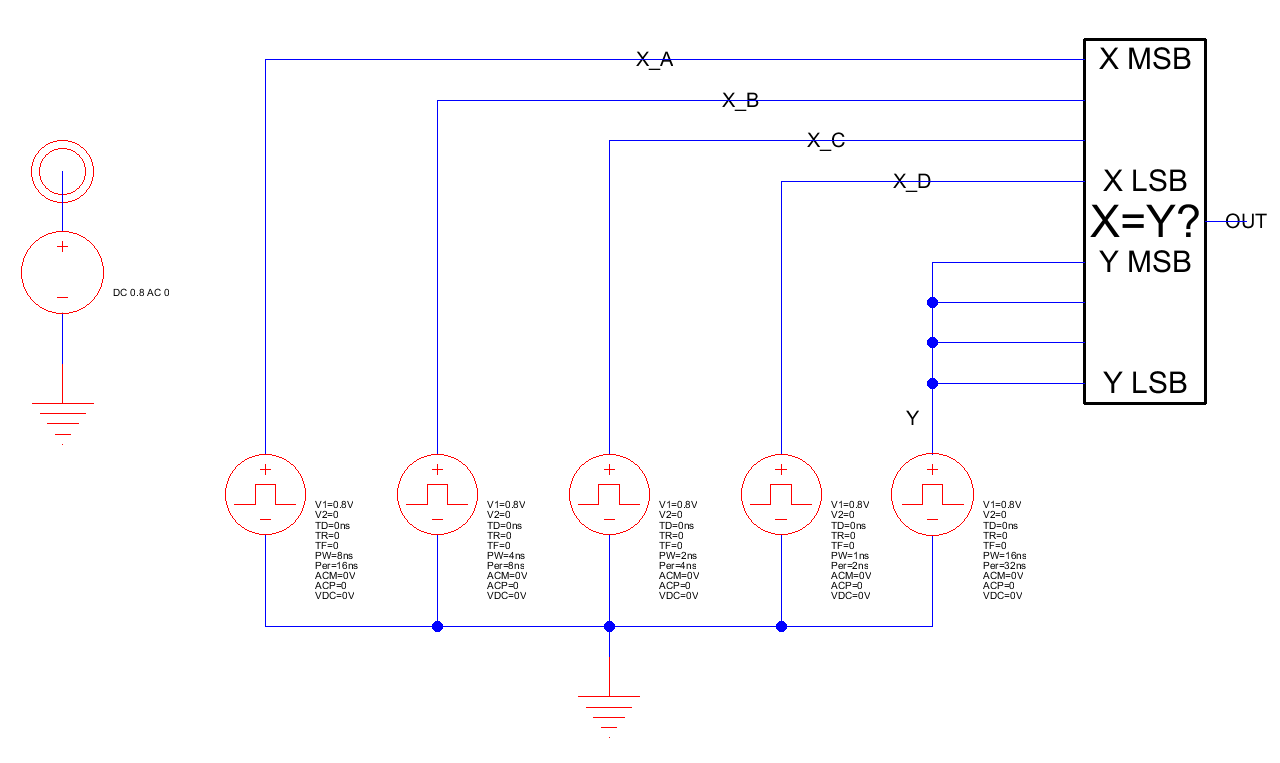
\includegraphics[width=1.0\textwidth]{TestSchematics/comparator.PNG}
  \caption{Comparator test schematic}
\end{figure}

\subsubsection*{D Latch}
\begin{figure}[H]
  \centering
    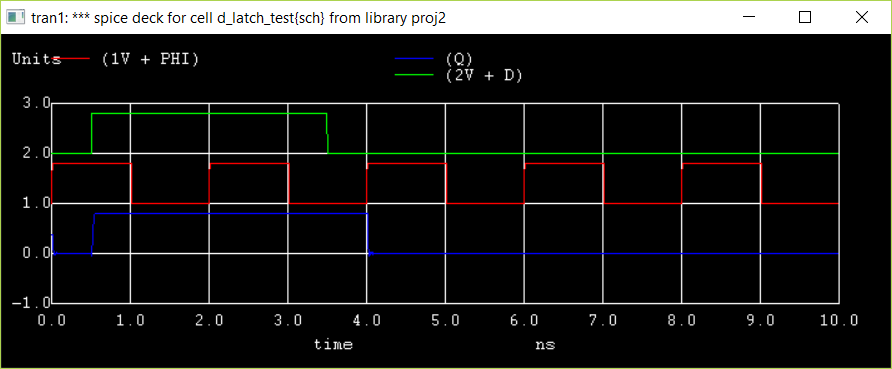
\includegraphics[width=1.0\textwidth]{d_latch_test.PNG}
  \caption{D Latch Test}
  \label{fig:d_latch_test}
\end{figure}
\begin{figure}[H]
  \centering
    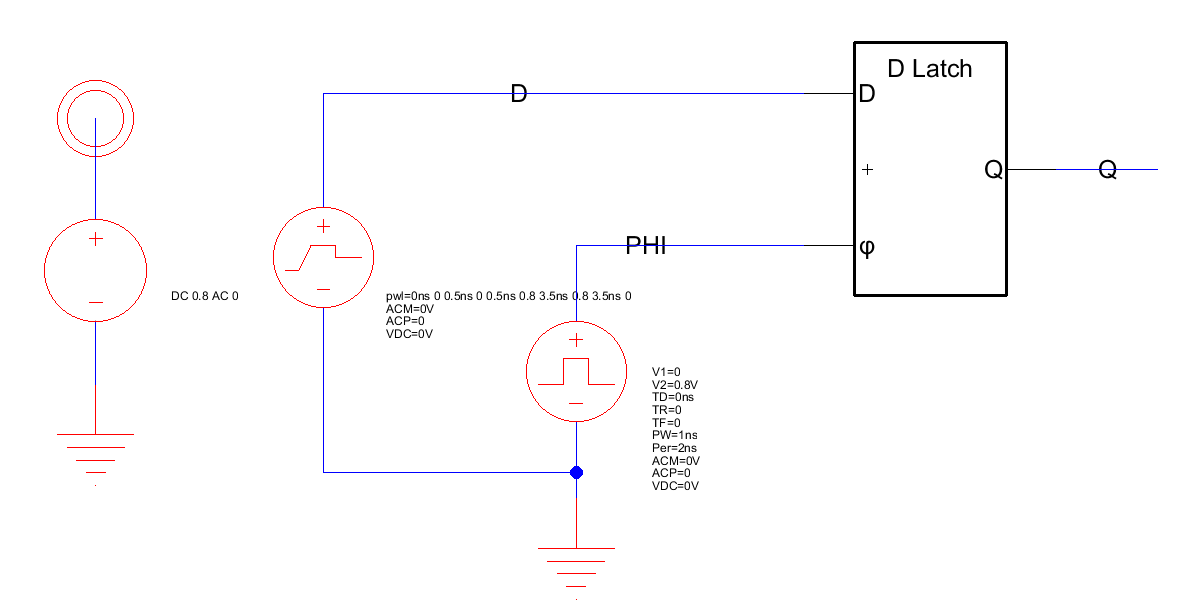
\includegraphics[width=1.0\textwidth]{TestSchematics/d_latch.PNG}
  \caption{D latch test schematic}
\end{figure}

\subsubsection*{D Register}
\begin{figure}[H]
  \centering
    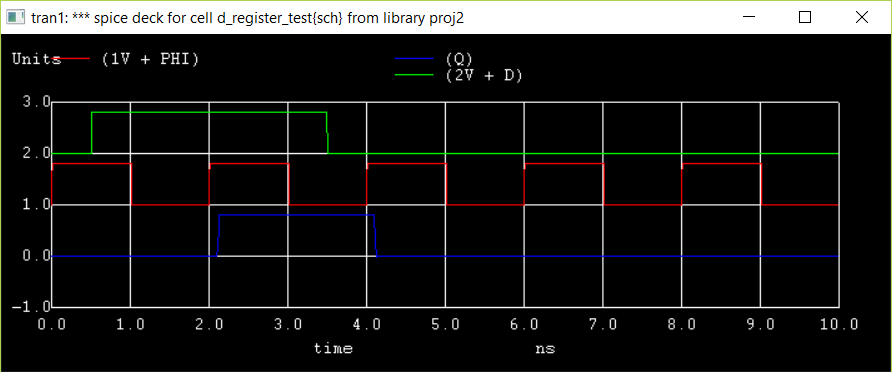
\includegraphics[width=1.0\textwidth]{d_register_test.PNG}
  \caption{D Register Test}
  \label{fig:d_register_test}
\end{figure}
\begin{figure}[H]
  \centering
    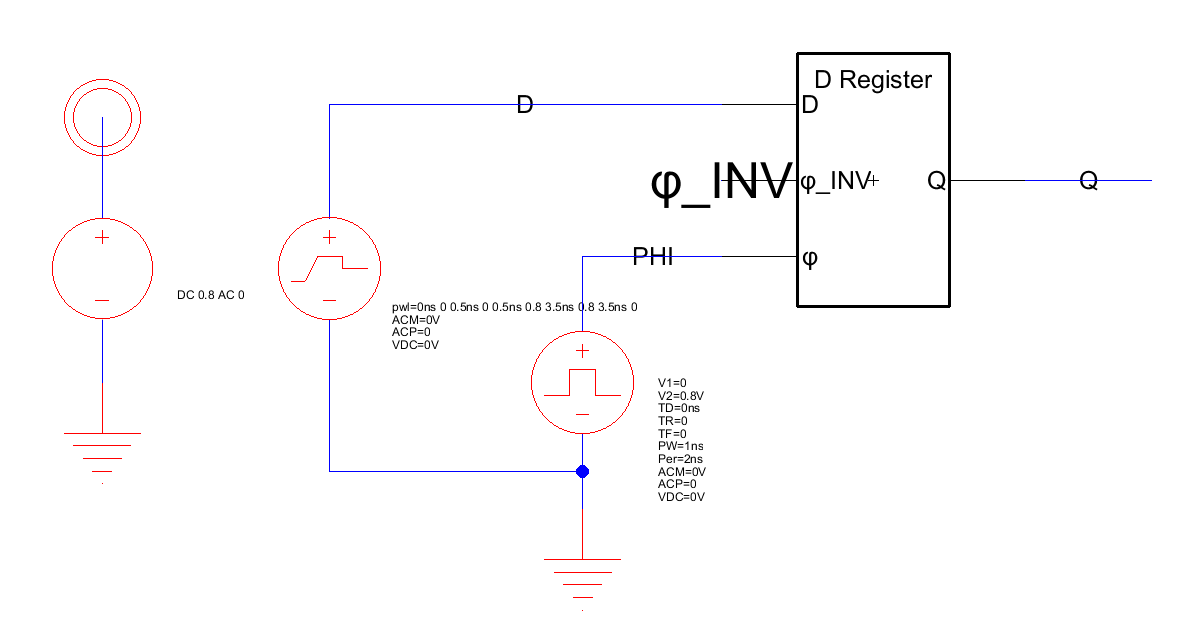
\includegraphics[width=1.0\textwidth]{TestSchematics/d_register.PNG}
  \caption{D register test schematic}
\end{figure}

\subsubsection*{ENQ*/DEQ* Module}
\begin{figure}[H]
  \centering
    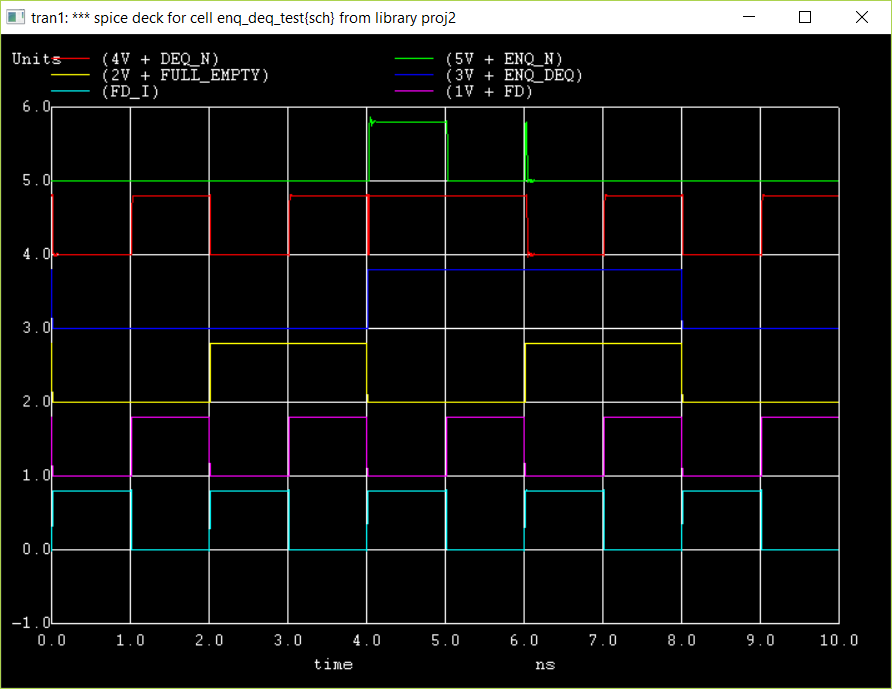
\includegraphics[width=1.0\textwidth]{enq_deq_test.PNG}
  \caption{ENQ*/DEQ* Module Test}
  \label{fig:enq_deq_test}
\end{figure}
\begin{figure}[H]
  \centering
    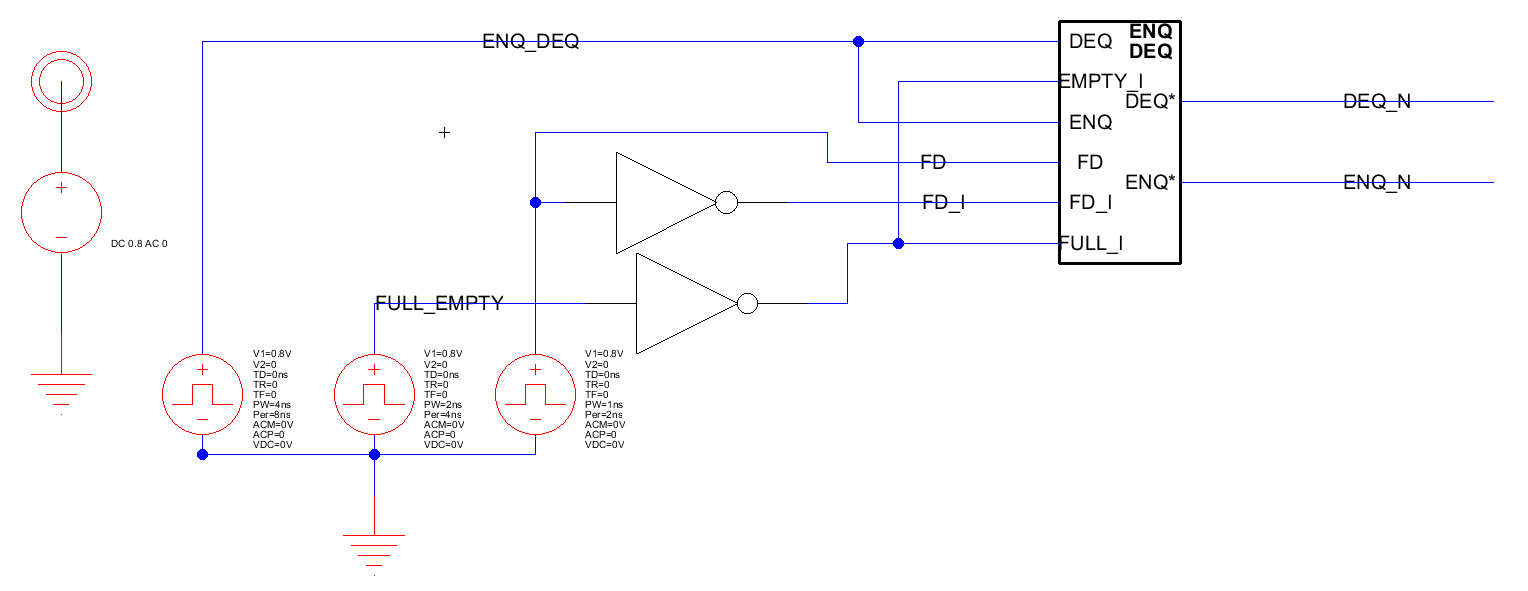
\includegraphics[width=1.0\textwidth]{TestSchematics/enq_deq.PNG}
  \caption{ENQ*/DEQ* test schematic}
\end{figure}

\subsubsection*{Incrementer}
\begin{figure}[H]
  \centering
    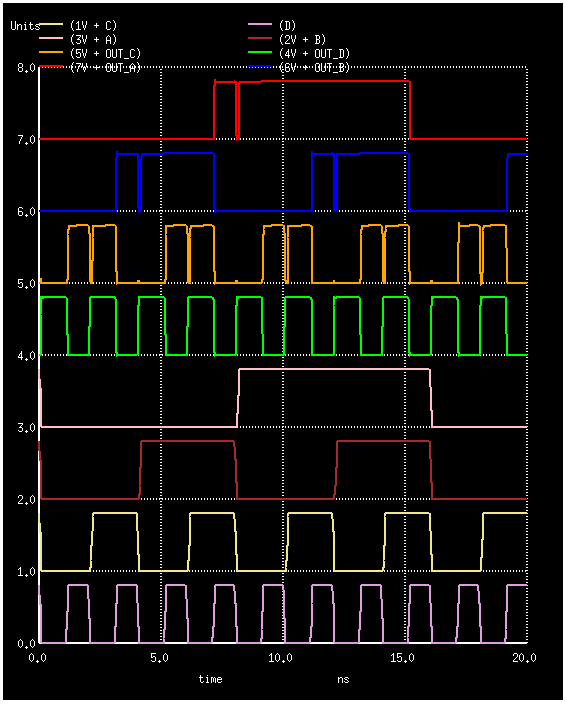
\includegraphics[width=1.0\textwidth]{incrementer_test.PNG}
  \caption{Incrementer Test}
  \label{fig:incrementer_test}
\end{figure}
\begin{figure}[H]
  \centering
    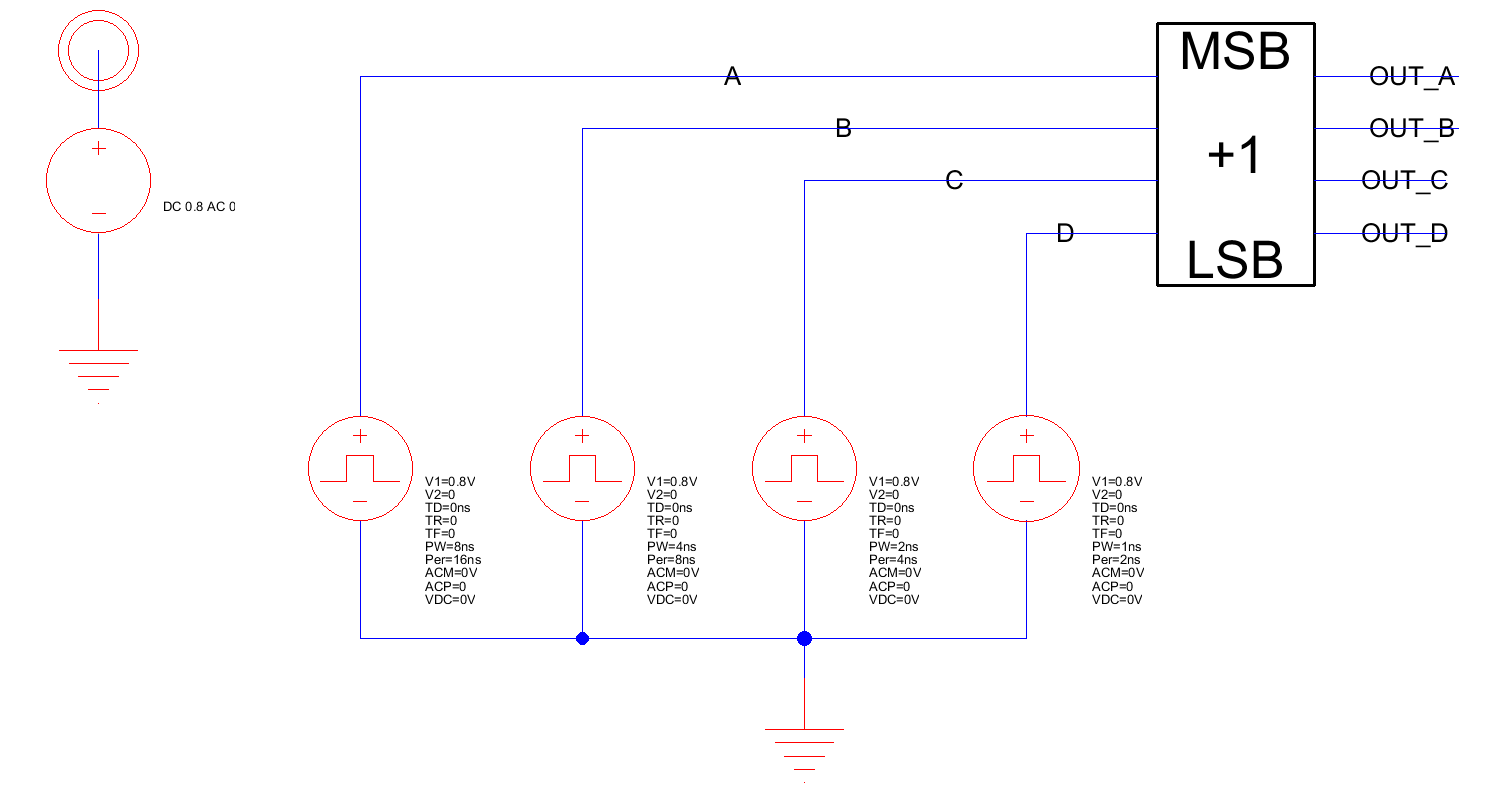
\includegraphics[width=1.0\textwidth]{TestSchematics/incrementer.PNG}
  \caption{Incrementer test schematic}
\end{figure}

\subsubsection*{Pointers}
The pointers test is broken down into testing for proper incrementing, testing for no incrementing when not enqueuing or dequeuing, and testing that the empty and full lines are asserted at the appropriate times (and not asserted when the queue is neither empty nor full (head != tail)).
\begin{figure}[H]
  \centering
    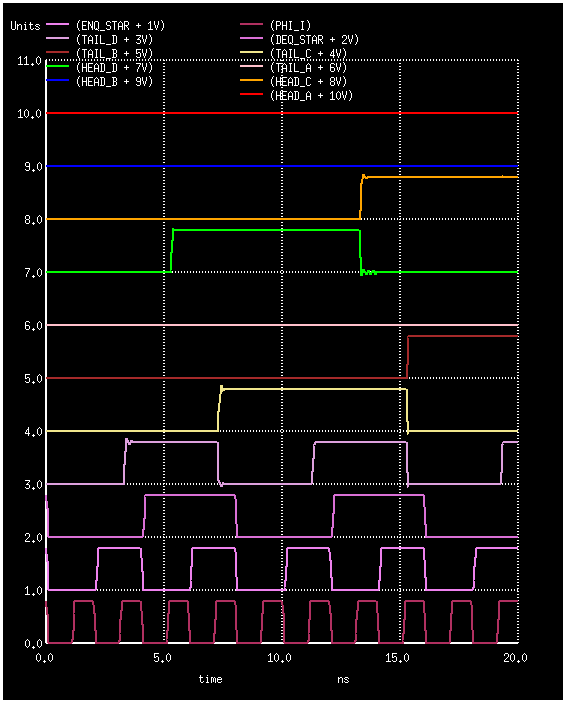
\includegraphics[width=1.0\textwidth]{pointers_test.PNG}
  \caption{Pointers test, proper increment}
  \label{fig:pointers_test}
\end{figure}
\begin{figure}[H]
  \centering
    \includegraphics[width=1.0\textwidth]{pointers_test_do_nothing.PNG}
  \caption{Pointers test, no incrementing}
  \label{fig:pointers_test_do_nothing}
\end{figure}
\begin{figure}[H]
  \centering
    \includegraphics[width=1.0\textwidth]{pointers_test_empty_full.PNG}
  \caption{Pointers test, empty and full}
  \label{fig:pointers_test_empty_full}
\end{figure}
\begin{figure}[H]
  \centering
    \includegraphics[width=1.0\textwidth]{TestSchematics/pointers.PNG}
  \caption{Pointers test schematic}
\end{figure}

\subsubsection*{Decoder}
\begin{figure}[H]
  \centering
    \includegraphics[width=1.0\textwidth]{decoder_test_0_to_3.PNG}
  \caption{Decoder test, outputs 0 to 3}
  \label{fig:decoder_test_0_to_3}
\end{figure}
\begin{figure}[H]
  \centering
    \includegraphics[width=1.0\textwidth]{decoder_test_4_to_7.PNG}
  \caption{Decoder test, outputs 4 to 7}
  \label{fig:decoder_test_4_to_7}
\end{figure}
\begin{figure}[H]
  \centering
    \includegraphics[width=1.0\textwidth]{decoder_test_8_to_11.PNG}
  \caption{Decoder test, outputs 8 to 11}
  \label{fig:decoder_test_8_to_11}
\end{figure}
\begin{figure}[H]
  \centering
    \includegraphics[width=1.0\textwidth]{decoder_test_12_to_15.PNG}
  \caption{Decoder test, outputs 12 to 15}
  \label{fig:decoder_test_12_to_15}
\end{figure}
\begin{figure}[H]
  \centering
    \includegraphics[width=1.0\textwidth]{TestSchematics/decoder.PNG}
  \caption{Decoder test schematic}
\end{figure}

\subsubsection*{Force Dequeue}
\begin{figure}[H]
  \centering
    \includegraphics[width=1.0\textwidth]{control_block_force_dequeue_test.PNG}
  \caption{Force dequeue module test}
  \label{fig:control_block_force_dequeue_test}
\end{figure}
\begin{figure}[H]
  \centering
    \includegraphics[width=1.0\textwidth]{TestSchematics/force_dequeue.PNG}
  \caption{Force dequeue test schematic}
\end{figure}

\subsubsection*{4-bit Precharge Module}
\begin{figure}[H]
  \centering
    \includegraphics[width=1.0\textwidth]{control_block_precharge_test.PNG}
  \caption{4-bit precharge module test}
  \label{fig:control_block_precharge_test}
\end{figure}
\begin{figure}[H]
  \centering
    \includegraphics[width=1.0\textwidth]{TestSchematics/precharge.PNG}
  \caption{4-bit precharge test schematic}
\end{figure}

\subsubsection*{Bitline Driver}
Note that we used resistors in our test circuit to drive the outputs of the tri-state buffers low after write-enable was disabled. We did not use resistors in our actual design.
\begin{figure}[H]
  \centering
    \includegraphics[width=1.0\textwidth]{control_block_bitline_driver_test_0.PNG}
  \caption{Bitline driver test, bit 0}
  \label{fig:control_block_bitline_driver_test}
\end{figure}
\begin{figure}[H]
  \centering
    \includegraphics[width=1.0\textwidth]{control_block_bitline_driver_test_1.PNG}
  \caption{Bitline driver test, bit 1}
  \label{fig:control_block_bitline_driver_test}
\end{figure}
\begin{figure}[H]
  \centering
    \includegraphics[width=1.0\textwidth]{control_block_bitline_driver_test_2.PNG}
  \caption{Bitline driver test, bit 2}
  \label{fig:control_block_bitline_driver_test}
\end{figure}
\begin{figure}[H]
  \centering
    \includegraphics[width=1.0\textwidth]{control_block_bitline_driver_test_3.PNG}
  \caption{Bitline driver test, bit 3}
  \label{fig:control_block_bitline_driver_test}
\end{figure}
\begin{figure}[H]
  \centering
    \includegraphics[width=1.0\textwidth]{TestSchematics/bitline_driver.PNG}
  \caption{Bitline driver test schematic}
\end{figure}

\subsection*{Full FIFO Queue}
For the full queue, we tested several operations.

The first operation that we tested is enqueueing once, then dequeueing twice. This was done to ensure that dequueing an empty queue does not result in the head or tail pointers changing. It also tests that we are dequeueing the correct value when we issue a valid dequeue request.

\begin{figure}[H]
  \centering
    \includegraphics[width=1.0\textwidth]{queue_toplevel_test_enq_deq_deq.PNG}
  \caption{Queue test, enqueue once and then dequeue twice}
\end{figure}

The second test we did was ensuring that enqueueing on a full queue does not result in the tail pointer changing.

\begin{figure}[H]
  \centering
    \includegraphics[width=1.0\textwidth]{queue_toplevel_test_enq_when_full.PNG}
  \caption{Queue test, enqueue on full queue}
\end{figure}

We also performed a test in which we enqueued and dequeued a few times. We first enqueue 1 and then enqueue 0 2 times. The first dequeue returns 1, and the next two dequeues return 0, as expected.

\begin{figure}[H]
  \centering
    \includegraphics[width=1.0\textwidth]{queue_toplevel_test_enq_deq_a_few_time.PNG}
  \caption{Queue test, enqueue and dequeue a few times}
\end{figure}

We also tested that enqueueing and dequeuing simultaneously worked according to the specifications. As shown, enq/deq on an empty queue just enqueues, while enq/deq on a non-empty, non-full queue does enqueue and dequeue a value.

\begin{figure}[H]
  \centering
    \includegraphics[width=1.0\textwidth]{queue_toplevel_test_enqdeq_empty_and_middle.PNG}
  \caption{Queue test, simultaneous enqueue and dequeue on empty and nonempty, nonfull}
\end{figure}

\newpage
\section*{Summary of Design Metrics}
The design metrics are summarized as follows:
\subsection*{Area}
Total area: 5892 (summing transistor widths). See breakdown below.
\subsection*{Memory Cell Area}
Area: 50

Areas are broken down as follows:\\

\begin{verbatim}
General Components
    Inverter: 2
    NAND Gate: 4
    AND2 Gate: 6
    NOR Gate: 4
    OR Gate: 6
    XOR Gate: 12
    XNOR Gate: 12
    AND4 Gate: 18
      3 AND2 Gates
    Tri-state Buffer: 38
    Tri-state Inverter: 38
    D Latch: 22
      1 inverter: 2
      2 AND2 gates: 12
      2 NOR gates: 8
    D Register: 46
      2 D latches: 44
      2 NMOS gates for reset: 2
    4-bit D Register: 184
      4 D registers
    Incrementer: 74
      6 AND2 Gates: 36
      2 OR Gates: 12
      2 NAND Gates: 8
      1 XOR Gate: 12
      3 inverters: 6
    Comparator: 66
      4 XNOR Gates: 48
      1 AND4 Gate: 18
    Mux Bitslice: 18
      2 AND2 Gates: 12
      1 OR2 Gate: 6
    Mux: 72
      4 Mux Bitslices
    Enq/Deq Module: 24
      3 AND2 Gates: 18
      1 OR2 Gate: 6
    WL Enable Module: 12
      1 OR2 Gate: 6
      1 AND2 Gate: 6
    Clock Generator: 58
      (directly in transistors)
    Force Dequeue: 52
      AND Gate: 6
      D Register: 46
    Pointers Module: 1108
      4 4-bit Registers: 736
      2 Incrementers: 148
      1 Comparator: 66
      1 D Register: 46
      2 AND4 Gates: 36
      11 AND2 Gates: 66
      1 OR2 Gate: 6
      2 Inverters: 4
    1-bit Bitline Precharge Module: 32
      2 PMOS Gates (W = 16): 32
    4-bit Bitline Precharge Module: 140
      4 1-bit Precharge Modules: 128
      1 NAND2 Gate: 4
      1 AND2 Gate: 6
      1 inverter: 2
    Bitline Driver Module: 350
      4 Tri-state Buffers: 152
      4 Tri-state Inverters: 152
      1 D Register: 46
    6T SRAM Cell: 50
      2 NMOS Gates (W = 8): 16
      2 NMOS Gates (W = 16): 32
      2 PMOS Gates (W = 1): 2
    4-to-16 Decoder: 392
      16 AND4 Gates: 288
      4 inverters: 8
      16 AND2 Gates: 96


Total Top-Level Design Area: 5892
    Control Block: 2284
      1 Clock Generator: 58
      1 Force Dequeue Module: 52
      1 Pointers Module: 1108
      2 4-bit Registers: 368
      1 Mux: 72
      1 Enq/Deq Module: 24
      1 WL Enable Module: 12
      1 4-bit Bitline Precharge Module: 140
      1 Bitline Driver Module: 350
      2 D Registers: 92
      4 inverters: 8
    Memory Block: 3592
      64 6T SRAM Cells: 3200
      1 4-to-16 Decoder: 392
    8 inverters for buffering: 16
\end{verbatim}

\subsection*{Enqueue Energy}
  Enqueueing 0x1111 into 0x0000: $4.78 x 10^{-14}$ J (higher value). This was done using the command 
  \begin{verbatim}
  meas tran yint integ I(vv_generi@0) from=36ns to=38ns
  \end{verbatim}
  and produced the results
  \begin{verbatim}
  yint = 5.97328e-14 from=  3.60000e-08 to=  3.80000e-08
  \end{verbatim}
  (Energy was multiplied by 0.8 since $V_{dd} = 0.8 $V.)

  Enqueueing 0x0000 into 0x1111: $4.73 x 10^{-14}$ J.
  \begin{verbatim}
  meas tran yint integ I(vv_generi@0) from=36ns to=38ns
  yint = -5.90996e-14 from=  3.60000e-08 to=  3.80000e-08
  \end{verbatim}
\subsection*{Dequeue Energy}
  Dequeueing 0x0000: $3.89 x 10^{-14}$ J (higher value).
  \begin{verbatim}
  yint = -4.86632e-014 from=  8.00000e-009 to=  1.00000e-008
  \end{verbatim}
  Dequeueing 0x1111: $3.818792 x 10^{-14}$ J 
  \begin{verbatim}
  yint = -4.77349e-014 from=  8.00000e-009 to=  1.00000e-008
  \end{verbatim}
\subsection*{Simultaneous Enqueue/Dequeue Energy}
  Result: $3.95 x 10^{-13}$ J
  \begin{verbatim}
  meas tran yint integ I(vv_generi@0) from=36ns to=40ns
  yint = -4.93721e-13 from=  3.60000e-08 to=  4.00000e-08
  \end{verbatim}
\subsection*{Standby Energy}
  Result:    $1.54 x 10^{-14}$ J 
  \begin{verbatim}
  yint = -1.93039e-014 from=  4.00000e-009 to=  6.00000e-009)
  \end{verbatim}
\subsection*{Average Energy}
  We calculated the average energy as a weighted average of the energies determined above and using the distribution specified in the report writeup. The average energy was $7.79 x 10^{-14}$ J and was calculated as $0.15 * 3.95 x 10^{-13} J + 0.1 * 4.78 x 10^{-14} + 0.1 * 3.89 x 10^{-14} J + 0.65 * 1.54 x 10^{-14}$ J

\newpage
\section*{Honor Pledge}
\begin{center}
\fbox{%
    \parbox{0.8\linewidth}{%
        We, Jack Harkins and Mauricio Mutai, certify that we have complied with the University of\\
        Pennsylvania's Code of Academic Integrity in completing this project.
    }%
}
\end{center}

\end{document}
